%%---------------------------------------------------------------------------%%
%%------------ 第二章:矩阵根的~Newton~法 -----------------------------------%%
%%---------------------------------------------------------------------------%%


\chapter{计算矩阵~$p$~次根的~Newton~法}
\label{chapter:NM_MatrixRoot}

我们把后文中用到的混合有限元方法和构建混合元所用的几何遗传树结构,以及移动网格方法,
在本章中做简要描述和历史回顾。

%Newton's method and Halley's method are the ones most widely used
%for computing the principal $p$th root $A^{1/p}$. Their iterative
%forms can be obtained by applying the corresponding classical forms
%to the matrix equation

应用迭代法计算矩阵的~$p$~次根, 实际上是求解如下的计算矩阵方程
\begin{equation}
\label{eq:f(X)=0} f(X) = X^p - A = 0, \quad p \geq 2.
\end{equation}
%Formally, Newton's method can be written as follows:
若假设初始迭代点~$X_0$~与矩阵~$A$~是可交换的, 且对于任意的~$k \geq
0$, $X_k$~都是非奇异的, 则计算上述矩阵方程的~Newton~法可写成:
\begin{equation}
\label{it:NM} X_{k+1}= N(X_k),\ \ \ k = 0,1,2,\ldots,
\end{equation}
%provided $X_0$ commutes with $A$ and that $X_k$ is nonsingular for
%any $k \geq 0$, where
其中
\begin{equation}
\label{it:NM_fun} N(X) := \frac{1}{p}X\left[(p-1)\I +
AX^{-p}\right].
\end{equation}


本章将研究通过~Newton~法来计算矩阵~$p$~次根的一个新的 收敛性结果。
新的结果比其他现有的结果在计算矩阵~$p$~次根时有更好的计算效果。
本章中总假定整数~$p \geq 2$.









%In this paper, we study refined convergence results on Newton's
%method and Halley's method for computing the principal $p$th root of
%a matrix. The new convergence regions which contain all the
%eigenvalues of $A$ guarantee (\ref{ineq:def_conv_order}) holds for
%all $k \geq 0$ for both methods. In Section 2 we will state our main
%results for both methods. And then the result concerning Newton's
%method will be proved in Section 3, while the one for Halley's
%method can be proved by using the similar approaches.





\section{收敛性结果}


在给出本章的主要收敛结果前, 先引入一些记号。令
\begin{equation}
\label{fun:phi(z)_NM} \phi_1(z) := 1 - u^p(z)(1 - z), \quad z \in
\MCD_{0,1},
\end{equation}
其中
\begin{equation*} u(z) := \frac{1}{1 - \frac{1}{p}z}, \quad z
\in \MCD_{0,1},
\end{equation*}
及
\begin{equation}
\label{set:D0_NM} \MCD_{0,1} := \left\{z \in \CS: |z| < p \right\}.
\end{equation}
定义
\begin{equation}
\label{set:R_NM} \MCR_1 := \left\{z\in \CS: 1 - z \in
\overline{\MCD}_1 \bigcup \left(\MCD_{0,1} \bigcap
\MCD_{2,1}\right)\right\}
\end{equation}
及
\begin{equation}
\label{set:R_hat_NM} \widehat{\MCR}_1 := \left\{z\in\CS: 1-z \in
\mathcal {D}_1 \bigcup \left(\mathcal {D}_{0,1} \bigcap \mathcal
{D}_{2,1}\right)\right\},
\end{equation}
其中~$\MCD_{0,1}$~由~(\ref{set:D0_NM})~给出, $\MCD_1$~定义为
\begin{equation}
\label{set:D1_NM} \MCD_1 := \{z \in \CS: |z| < 1\},
\end{equation}
$\overline{\MCD}_1$~为~$\MCD_1$~的闭包, 而
\begin{equation}
\label{set:D2_NM} \MCD_{2,1} := \left\{z \in \CS: \sup_{m \geq 2}
\left\{\frac{|S_{1,m}(z)|}{|z|}\right\} \cdot \frac{|z|
+|\phi_1(z)|}{\big||z| - |\phi_1(z)|\big|} < 1 \right\},
\end{equation}
其中~$\phi_\nu$~ 由~(\ref{fun:phi(z)_NM})~给出,
\begin{equation}
\label{ser:Sm(z)_NM} S_{1,m}(z) = \sum\limits_{j = 2}^{m} c_{1,j}
z^{j}, \quad z \in \MCD_{0,1},
\end{equation}
其中
\begin{equation*}
\label{cons:NM_c1j} c_{1,j} =
\frac{p(p+1)\cdot(p+j-2)}{(j-1)!p^{j-1}} -
\frac{p(p+1)\cdot(p+j-1)}{j!p^j} > 0, \quad j=2,3,\ldots,
\end{equation*}
并满足
$$
\sum_{j=2}^\infty c_{1,j}=1,
$$
故 ~$\phi_1(z)$ 有如下的~Maclaurin~级数形式
\begin{equation}
\label{fun:phi1(z)_series} \phi_1(z) = \sum_{j=2}^\infty c_{1,j}
z^j, \quad z \in \MCD_{0,1},
\end{equation}
其中 ~$\MCD_{0,1}$~ 由 ~(\ref{set:D0_NM})~给出.



下面给出应用~Newton~法~(\ref{it:NM})~来计算矩阵主~$p$~次根时的收敛性结果:


\begin{theorem}
\label{th:MatrixNMCon} 设~$\MCR_1$~由~$(\ref{set:R_NM})$~定义,
而~$\widehat{\MCR}_1$~ 由~$(\ref{set:R_hat_NM})$~定义。 如果矩阵~$A
\in \CS^{n \times n}$~的所有特征值都属于~$\MCR_1$~
且所有零特征值都是半单的, 那么以~$X_0 =
\I$~为初始点的~Newton~法~$(\ref{it:NM})$~迭代所产生的矩阵序列~$\{X_k\}$~收敛于
矩阵~$A$~的主~$p$~次根~$A^{1/p}$。特别地,
如果~$A$~的所有特征值都属于~$\widehat{\MCR}_1\backslash\{0\}$,
那么~Newton~法~$(\ref{it:NM})$~是二次收敛的。
\end{theorem}

\begin{remark}
图~\ref{fig:NM_ConvReg}~所示的是,
由~(\ref{set:R_NM})~所定义的~$\MCR_1$~ 的近似收敛域的九种情形,
其中红色表示的是收敛域~$\{z \in \CS: 1-z \in \overline{\MCD}_1\}$,
而蓝色表示的是收敛域~$\{z\in \CS: 1-z \in
\MCD_{0,1}\bigcap\MCD_{2,1}\}$。由该图可知, 对于某一固定的~$p$,
当~$m$~分别取 ~$m=20, 100, 500$~时,
所得到的近似收敛域~(见~(a)-(c),或 ~(d)-(f), 或
~(g)-(i))~几乎一样。为此, 在实际计算中只需要取~$m=20$~即可。
\end{remark}

\begin{figure}[h!]
\centering
\subfigure[]{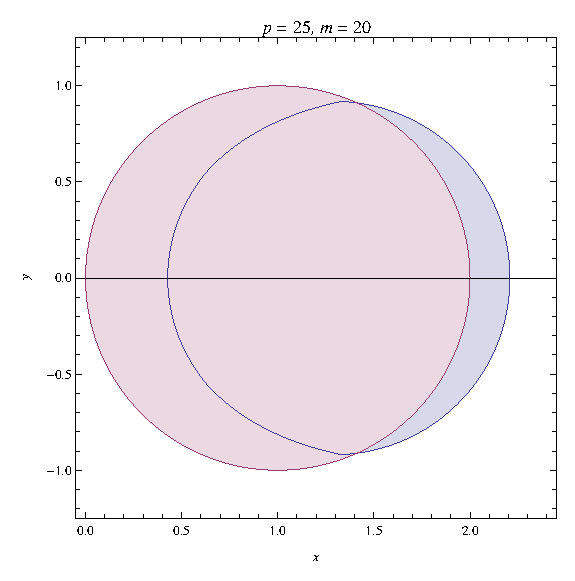
\includegraphics[width=0.3\textwidth]{fig_NM_ConvReg_p25m20.eps}}
\subfigure[]{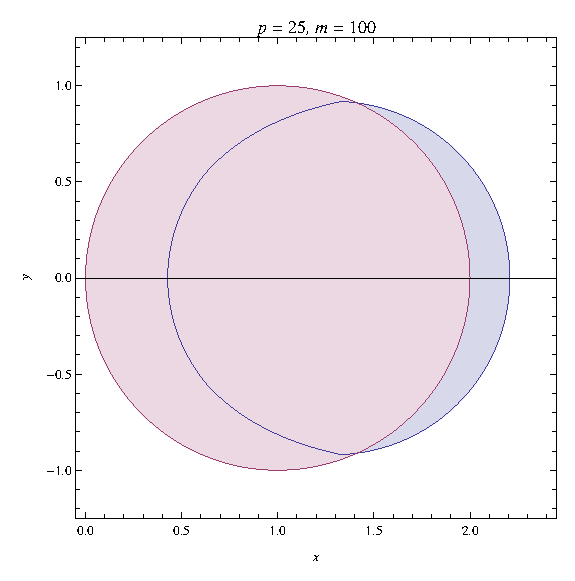
\includegraphics[width=0.3\textwidth]{fig_NM_ConvReg_p25m100.eps}}
\subfigure[]{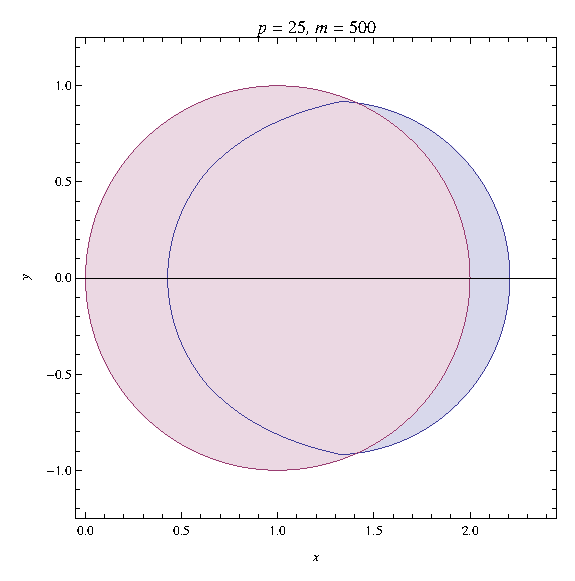
\includegraphics[width=0.3\textwidth]{fig_NM_ConvReg_p25m500.eps}}\\
\subfigure[]{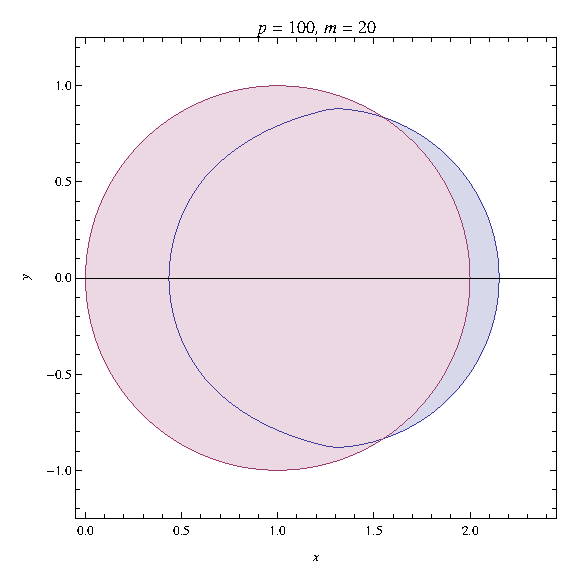
\includegraphics[width=0.3\textwidth]{fig_NM_ConvReg_p100m20.eps}}
\subfigure[]{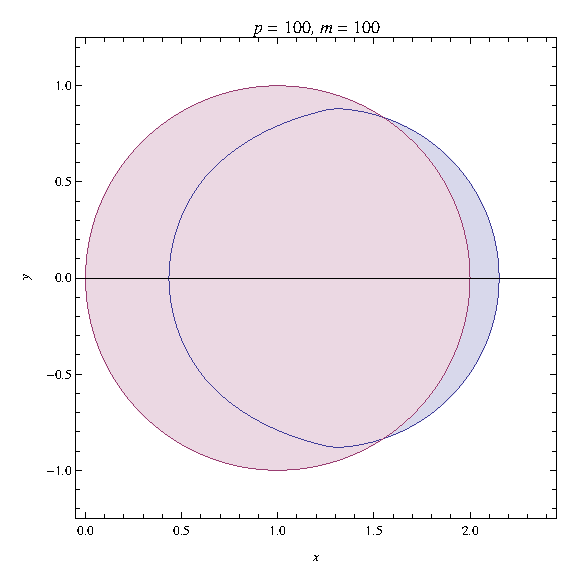
\includegraphics[width=0.3\textwidth]{fig_NM_ConvReg_p100m100.eps}}
\subfigure[]{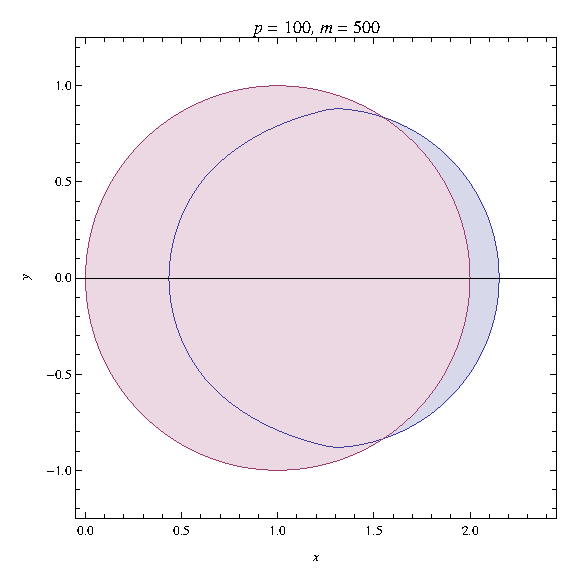
\includegraphics[width=0.3\textwidth]{fig_NM_ConvReg_p100m500.eps}}\\
\subfigure[]{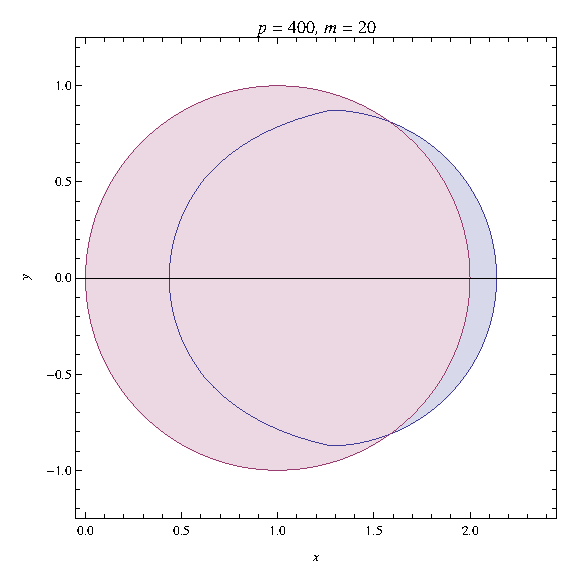
\includegraphics[width=0.3\textwidth]{fig_NM_ConvReg_p400m20.eps}}
\subfigure[]{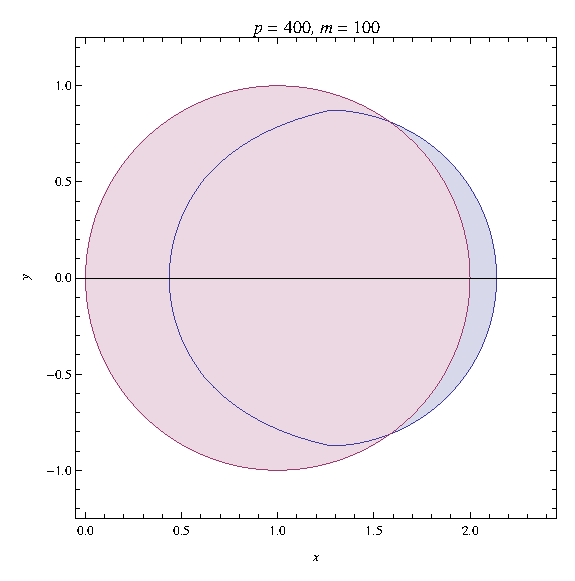
\includegraphics[width=0.3\textwidth]{fig_NM_ConvReg_p400m100.eps}}
\subfigure[]{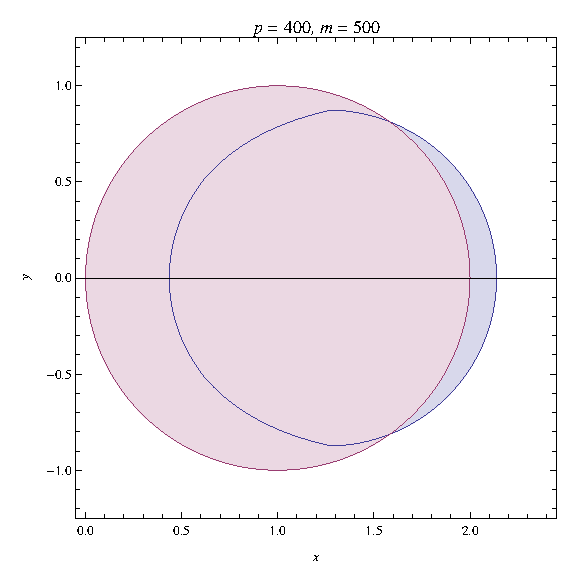
\includegraphics[width=0.3\textwidth]{fig_NM_ConvReg_p400m500.eps}}\\
%\caption{The approximating regions of $\MCR_1$ defined in
%(\ref{set:R_NM}) for $p = 25, 100, 400$ and $m = 20, 100, 500$,
%where the red and blue regions denote the sets $\{z\in\CS: 1-z \in
%\overline{\MCD}_1\}$ and $\{z\in \CS: 1-z \in \MCD_{0,1} \bigcap
%\MCD_{2,1}\}$, respectively. }
\caption{由~(\ref{set:R_NM})~给出的~$\MCR_1$~在九种不同情形~($p$~分别取~25,
100, 400~及~$m$~分别取~20, 100, 500)~下的近似域,
其中红色域表示集合~$\{z\in\CS: 1-z \in \overline{\MCD}_1\}$},
而蓝色域表示集合~$\{z\in \CS: 1-z \in \MCD_{0,1}
\bigcap\MCD_{2,1}\}.$\label{fig:NM_ConvReg}
\end{figure}















%\section{定理~\ref{th:MatrixNMCon}~的证明}


%In this section, we will prove in detail Theorem
%\ref{th:MatrixNMCon}, the results on convergence and convergence
%order for Newton's method (\ref{it:NM}). Theorem
%\ref{th:MatrixHMCon} for Halley's method (\ref{it:HM}) can be
%similarly proved by using the analysis approaches. We omit the
%details.



\section{预备引理}

在证明定理~\ref{th:MatrixNMCon}~前, 需要一些有用的预备引理.

给定任意一个复数~$\lambda \in \CS$, 令

%For a complex number $\lambda \in \CS$, let
\begin{equation}
\label{fun:f(z)} f(z) := z^p - \lambda, \ \ \ z \in \CS
\end{equation}
及
\begin{equation}
\label{fun:r(z)} r(z,\lambda) := 1 - \lambda z^{-p}, \ \ \ z \in
\CS\backslash\{0\}.
\end{equation}

\begin{lemma}
\label{lem:NM_r(N(z))_r(z)} 设~$r(z,\lambda)$~由~$(\ref{fun:r(z)})$~
定义. 对于某个复数~$z \in \CS\backslash\{0\}$, 若~$r(z,\lambda) \in
\mathcal {D}_{0,1}\backslash\{1\}$,
其中~$\MCD_{0,1}$~由~$(\ref{set:D0_NM})$~给出,
则由~$(\ref{it:NM_fun})$~的标量形式所得到的~$N(z)$~有定义且
\begin{equation}
\label{eq:r(N(z))_1} r(N(z),\lambda) = \phi_1(r(z,\lambda)),
\end{equation}
其中~$\phi_1(z)$~由~$(\ref{fun:phi(z)_NM})$~定义. 此外,
有如下的估计: 当~$r(z,\lambda) \in
\overline{\MCD}_1\backslash\{0,1\}$~时,
\begin{equation}
\label{ineq:abs_r(N(z))_1} |r(N(z),\lambda)| < |r(z,\lambda)|^2.
\end{equation}
当~$r(z,\lambda) \in \mathcal {D}_{0,1}\backslash\{1\}$~时,
\begin{equation}
\label{ineq:abs_r(N(z))_2} |r(N(z),\lambda)| \leq \sup_{m \geq
2}\left\{\left|\frac{S_{1,m}(u)}{u^2}\right|\right\}\cdot \frac{|u|
+ |r(z,\lambda)|}{|u| - |r(z,\lambda)|} \cdot |r(z,\lambda)|^2,
\end{equation}
其中~$\overline{\MCD}_1$~为~$\MCD_1$~的闭包,
而~$\MCD_1$~由~$(\ref{set:D1_NM})$~定义,
$S_{1,m}(u)$~由~$(\ref{ser:Sm(z)_NM})$~定义且对于每一个~$u \in
\MCD_{0,1}$~均满足~$|u| > |r(z,\lambda)|$, $m \geq 2$.
\end{lemma}

%\begin{lemma}
%\label{lem:NM_r(N(z))_r(z)} Let $r(z,\lambda)$ be defined in
%$(\ref{fun:r(z)})$. If $r(z,\lambda) \in \mathcal
%{D}_{0,1}\backslash\{1\}$ for some $z \in \CS\backslash\{0\}$, where
%$\MCD_{0,1}$ is defined in $(\ref{set:D0_NM})$, then $N(z)$
%generated by the scalar case of $(\ref{it:NM_fun})$ for $f(z)$
%defined in $(\ref{fun:f(z)})$ exists and
%\begin{equation}
%\label{eq:r(N(z))_1} r(N(z),\lambda) = \phi_1(r(z,\lambda)),
%\end{equation}
%where $\phi_1(z)$ is defined by $(\ref{fun:phi(z)_NM})$. Moreover,
%we have
%\begin{numcases}{}
%|r(N(z),\lambda)| < |r(z,\lambda)|^2, &
%if \ $r(z,\lambda) \in \overline{\MCD}_1\backslash\{0,1\}$,\ \ \ \label{ineq:abs_r(N(z))_1}\\
%|r(N(z),\lambda)| \leq \sup_{m \geq
%2}\left\{\left|\frac{S_{1,m}(u)}{u^2}\right|\right\}\cdot \frac{|u|
%+ |r(z,\lambda)|}{|u| - |r(z,\lambda)|} \cdot |r(z,\lambda)|^2, &
%if \ $r(z,\lambda) \in \mathcal {D}_{0,1}\backslash\{1\}$,
%\label{ineq:abs_r(N(z))_2}
%\end{numcases}
%where $\overline{\MCD}_1$ is the closure of $\MCD_1$ defined in
%$(\ref{set:D1_NM})$, and $S_{1,m}(u)$ is given in
%$(\ref{ser:Sm(z)_NM})$ for each $u \in \MCD_{0,1}$ satisfying $|u| >
%|r(z,\lambda)|$, $m \geq 2$.
%\end{lemma}


\begin{proof}

%For any $z \in \CS\backslash\{0\}$, $N(z)$ exists by
%(\ref{it:NM_fun}). Note that

对于任意的复数~$z \in \CS\backslash\{0\}$,
由~(\ref{it:NM_fun})~知~$N(z)$~是存在的. 由于

\begin{equation}
\label{eq:N(z)} N(z) = \frac{1}{p}z\left[(p-1)+\lambda z^{-p}\right]
= z\left[1+\frac{1}{p}r(z,\lambda)\right] \neq 0.
\end{equation}
%It follows that
故
\begin{equation}
\label{eq:r(N(z))} r(N(z),\lambda) =
1-\left[1+\frac{1}{p}r(z,\lambda)\right]^{-p}(1-r(z,\lambda)) =
\phi_1(r(z,\lambda)),
\end{equation}
%which shows (\ref{eq:r(N(z))_1}) holds.
即得~(\ref{eq:r(N(z))_1})~是成立的.

%If $r(z,\lambda) \in \overline{\MCD}_1\backslash\{0,1\} \subset
%\MCD_{0,1}$, then, by (\ref{fun:phi1(z)_series}) and
%(\ref{eq:r(N(z))}), one has that

若~$r(z,\lambda) \in \overline{\MCD}_1\backslash\{0,1\} \subset
\MCD_{0,1}$, 则由~(\ref{fun:phi1(z)_series})~及~(\ref{eq:r(N(z))}),
并注意到对于任意的~$w \in \overline{\MCD}_1\backslash\{1\}$,
不等式~$|c_3 + c_4 w| < c_3 + c_4$~都是成立的, 于是可得
\begin{align}
|r(N(z),\lambda)| & = |\phi(r(z,\lambda))| \nonumber\\
& = |r(z,\lambda)|^2 \left| \sum_{j =
2}^\infty c_{1,j} r^{j-2}(z,\lambda) \right| \nonumber\\
& \leq |r(z,\lambda)|^2 \left[|c_{1,3} + c_{1,4} r(z,\lambda)| +
\sum_{j = 4}^\infty c_{1,j} |r(z,\lambda)|^{j-2}
\right] \nonumber\\
& < |r(z,\lambda)|^2 \sum_{j = 2}^\infty c_{1,j} =
|r(z,\lambda)|^2\nonumber\\
& \leq |r(z,\lambda)|. \label{ineq:abs_r(N(z))}
\end{align}
%from the fact that $|c_3 + c_4 w| < c_3 + c_4$ for all $w \in
%\overline{\MCD}_1\backslash\{1\}$. Thus, (\ref{ineq:abs_r(N(z))_1})
%is proved.
即~(\ref{ineq:abs_r(N(z))_1})~是成立的.


%If $r(z,\lambda) \in \mathcal {D}_0\backslash\{1\}$, based on
%(\ref{fun:phi1(z)_series}) and (\ref{eq:r(N(z))}) again, we have

若~$r(z,\lambda) \in \mathcal {D}_0\backslash\{1\}$,
则由~(\ref{fun:phi1(z)_series})~及~(\ref{eq:r(N(z))})~可知,
对于任意的 ~$u \in \CS\backslash\{0\}$~有
\begin{align*}
r(N(z),\lambda) & = \phi_1(r(z,\lambda))\\
& = \sum_{j=2}^\infty c_{1,j} r^j(z,\lambda)\\
& = \left[\sum_{j=2}^\infty c_{1,j} u^{j-2}
\left(\frac{r(z,\lambda)}{u}\right)^{j-2}\right] \cdot
r^2(z,\lambda).
\end{align*}
%holds for any $u \in \CS\backslash\{0\}$. Since, for any $m \geq 2$,
对于任意的~$m \geq 2$, 应用~Abel~变换可得
\begin{align*}
\sum_{j=2}^m c_{1,j} u^{j-2}
\left(\frac{r(z,\lambda)}{u}\right)^{j-2} & = \sum_{j=2}^{m-1}
\left(\sum_{\ell=2}^j c_{1,\ell} u^{\ell-2}\right)\left(1 -
\frac{r(z,\lambda)}{u}\right)\left(\frac{r(z,\lambda)}{u}\right)^{j-2}\\
& \ \ \ + \left(\sum_{\ell = 2}^m c_{1,\ell} u^{\ell-2}\right)\cdot
\left(\frac{r(z,\lambda)}{u}\right)^{m-2}.
\end{align*}
%by Abel transformation, we have
于是
\begin{align*}
\left|\sum_{j=2}^m c_{1,j} u^{j-2}
\left(\frac{r(z,\lambda)}{u}\right)^{j-2}\right| & \leq \sup_{2\leq
j \leq m-1} \left\{\left|\sum_{\ell=2}^j c_{1,\ell}
u^{\ell-2}\right|\right\} \cdot \left|1 -
\frac{r(z,\lambda)}{u}\right| \cdot \sum_{j=2}^{m-1}
\left|\frac{r(z,\lambda)}{u}\right|^{j-2}\\
& \ \ \ + \left|\frac{S_{1,m}(u)}{u^2} \right|\cdot
\left|\frac{r(z,\lambda)}{u}\right|^{m-2}, \quad m >2.
\end{align*}
%Then, letting $m \to \infty$ in the above inequality, it follows
%that
在上述不等式中令~$m \to \infty$, 则对于任意的~$r(z,\lambda) \in
\mathcal {D}_0\backslash\{1\}$~及满足关系~$|u|
> |r(z,\lambda)|$~的任意复数~$u
\in \mathcal {D}_0$, 有
\begin{align*}
|r(E(z),\lambda)| & \leq \sup_{m \geq 2} \left\{\left|\sum_{j=2}^m
c_{1,j} u^{j-2}\right|\right\} \cdot \left|1 -
\frac{r(z,\lambda)}{u}\right| \cdot
\sum_{m=2}^\infty \left|\frac{r(z,\lambda)}{u}\right|^{m-2}\cdot |r(z,\lambda)|^2 \\
& = \sup_{m \geq 2}
\left\{\left|\frac{S_{1,m}(u)}{u^2}\right|\right\} \cdot
\frac{\left|1 - \frac{r(z,\lambda)}{u}\right|}{1 -
\left|\frac{r(z,\lambda)}{u}\right|} \cdot |r(z,\lambda)|^2 \\
& = \sup_{m \geq 2}
\left\{\left|\frac{S_{1,m}(u)}{u^2}\right|\right\} \cdot \frac{|u| +
|r(z,\lambda)|}{|u| - \left|r(z,\lambda)\right|} \cdot
|r(z,\lambda)|^2.
\end{align*}
%for any $r(z,\lambda) \in \mathcal {D}_0\backslash\{1\}$ and any $u
%\in \mathcal {D}_0$ subject to $|u|
%> |r(z,\lambda)|$, which verifies (\ref{ineq:abs_r(N(z))_2}). The
%proof is completed.
从而~(\ref{ineq:abs_r(N(z))_2})~得证. 证完.
\end{proof}



\begin{lemma}
\label{lem:NM_r(z)_convergence1} %Let $r(z,\lambda)$ be defined in
%$(\ref{fun:r(z)})$. If $r(z_0,\lambda) \in
%\overline{\MCD}_1\backslash\{0,1\}$ for some $z_0 \in
%\CS\backslash\{0\}$, then the sequence $\{z_k\}$ starting from $z_0$
%generated by the scalar case of $(\ref{it:NM})$ for solving
%$(\ref{fun:f(z)})$ exists,

设~$r(z,\lambda)$~由~$(\ref{fun:r(z)})$~定义. 对于某个复数~$z_0 \in
\CS\backslash\{0\}$, 若~$r(z_0,\lambda) \in
\overline{\MCD}_1\backslash\{0,1\}$,
则由~$(\ref{it:NM})$~的标量形式~$($以~$z_0$~为初始点$)$~迭代产生的序列~$\{z_k\}$~
是有定义的, 且有估计式:
\begin{equation}
\label{ineq:NM_abs_r(zk)_1} |r(z_k,\lambda)| \leq
q_1^{2^{k-1}}(z_0), \ \ \ k = 1, 2, \ldots,
\end{equation}
%where
其中
\begin{equation}
\label{cons:NM_q1(z0)} q_1(z_0) = q_1(z_0,\lambda) :=
\left|\sum_{j=2}^\infty c_{1,j} r^{j-1}(z_0,\lambda)\right| < 1.
\end{equation}
%and so $|r(z_k,\lambda)| \to 0$ with order $2$ as $k \to \infty$.
由此可知, 当~$k \to \infty$~时~$|r(z_k,\lambda)|$~收敛于~0,
且收敛速度是二阶的.
\end{lemma}

\begin{proof}
%For $z_0$ chosen, $q_1(z_0) < 1$ follows from the same arguments
%used in (\ref{ineq:abs_r(N(z))}). By (\ref{ineq:abs_r(N(z))_1}) in
%Lemma \ref{lem:NM_r(N(z))_r(z)}, $z_1 = E(z_0)$ exists and

对于给定的~$z_0$,
类似于~(\ref{ineq:abs_r(N(z))})~的处理方式可知~$q_1(z_0) < 1$.
根据引理~\ref{lem:NM_r(N(z))_r(z)}~中的~(\ref{ineq:abs_r(N(z))_1})~知~$z_1
= E(z_0)$~是存在的并且有
$$
|r(z_1,\lambda)| = q_1(z_0)|r(z_0,\lambda)| \leq q_1(z_0) < 1.
$$
%Suppose that $z_k$ exists and (\ref{ineq:NM_abs_r(zk)_1}) holds for
%some $k \geq 1$, then by Lemma \ref{lem:NM_r(N(z))_r(z)} again,
%$z_{k+1} = E(z_k)$ exists and
对于某一~$k \geq 1$,
假设~$z_k$~是存在的且~(\ref{ineq:NM_abs_r(zk)_1})~是成立的,
则由引理~\ref{lem:NM_r(N(z))_r(z)}~可知~$z_{k+1} =
E(z_k)$~是存在的并且有
\begin{equation*}
|r(z_{k+1},\lambda)| < |r(z_{k},\lambda)|^2 \leq
\left[q_1^{2^{k-1}}(z_0)\right]^2 = q_1^{2^{k}}(z_0).
\end{equation*}
%Thus, (\ref{ineq:NM_abs_r(zk)_1}) holds for $k+1$. By induction,
%$\{z_k\}$ exists and (\ref{ineq:NM_abs_r(zk)_1}) holds. Furthermore,
%$r(z_k,\lambda) \to 0$ with order 2 as $k \to \infty$, which
%completes the proof.
由此知, (\ref{ineq:NM_abs_r(zk)_1})~对于~$k+1$~的情形仍然成立.
于是由归纳法知,
序列~$\{z_k\}$~是存在的且~(\ref{ineq:NM_abs_r(zk)_1})~恒成立. 证完.
\end{proof}



%The following lemma says that, besides in $
%\overline{\MCD}_1\backslash\{0,1\}$, it also guarantees
%$r(z_k,\lambda)$ converges quadratically to 0 as $k \to \infty$ when
%$r(z_0,\lambda) \in \MCD_{2,1} \bigcap \MCD_{0,1}\backslash\{1\}$
%for some $z_0 \in \CS\backslash\{0\}$.

对于某个复数~$z_0 \in \CS\backslash\{0\}$,
引理~\ref{lem:NM_r(z)_convergence1}~ 说明当~$r(z_0,\lambda) \in
\overline{\MCD}_1\backslash\{0,1\}$~时可保证~$r(z_k,\lambda)$~是二阶收敛于~0,
下面的引理表明, 除此之外, 当~$r(z_0,\lambda) \in \MCD_{2,1} \bigcap
\MCD_{0,1}\backslash\{1\}$~时,
仍然可以保证~$r(z_k,\lambda)$~是二阶收敛于~0.

\begin{lemma}
\label{lem:NM_r(z)_convergence2} %For any $z_0 \in
%\CS\backslash\{0\}$ satisfying $r(z_0,\lambda) \in \MCD_{2,1}
%\bigcap \MCD_{0,1}\backslash\{1\}$ and

设~$r(z,\lambda)$~由~$(\ref{fun:r(z)})$~定义. 对于某一复数~$z_0 \in
\CS\backslash\{0\}$, 若~$r(z_0,\lambda) \in \MCD_{2,1} \bigcap
\MCD_{0,1}\backslash\{1\}$~且
\begin{equation}
\label{cons:NM_q2(z0)} q_2(z_0) = q_2(z_0,\lambda) := \sup_{m \geq
2} \left\{\frac{|S_{1,m}(r(z_0,\lambda))|}{|r(z_0,\lambda)|}\right\}
\cdot \frac{|r(z_0,\lambda)|
+|\phi_1(r(z_0,\lambda))|}{|r(z_0,\lambda)| -
|\phi_1(r(z_0,\lambda))|} < 1,
\end{equation}
%where $\MCD_{2,1}$ is defined in $(\ref{set:D2_NM})$, the sequence
%$\{z_k\}$ generated by the scalar form of $(\ref{it:NM})$ starting
%from $z_0$ for solving $(\ref{fun:f(z)})$ exists,
其中~$\MCD_{2,1}$~由~$(\ref{set:D2_NM})$~定义,
则由~$(\ref{it:NM})$~的标量形式~$($以~$z_0$~为初始点$)$~
迭代产生的序列~$\{z_k\}$~是有意义的,
且有如下估计:
\begin{equation}
\label{ineq:NM_abs_r(zk)_2} |r(z_k,\lambda)| \leq q_2^{2^k-1}(z_0)
\cdot |r(z_0,\lambda)|, \quad k = 0, 1, \ldots.
\end{equation}
%and so $|r(z_k,\lambda)| \to 0$ with order $2$ as $k \to \infty$.
由此可知, 当~$k \to \infty$~时~$|r(z_k,\lambda)|$~收敛于~$0$,
且收敛速度是二阶的.
\end{lemma}

\begin{proof}
%For $z_0$ chosen, we have $r(z_0,\lambda) \in \mathcal
%{D}_{0,1}\backslash\{1\}$. So, $z_1 = N(z_0)$ exists and $z_1 \neq
%0$ by (\ref{eq:N(z)}). Recall that $S_{1,m}(r(z_0,\lambda)) \to
%\phi_1(r(z_0,\lambda))$ as $k\to\infty$ implies
显然, 对于给定的~$z_0$~有~$r(z_0,\lambda) \in \mathcal
{D}_{0,1}\backslash\{1\}$. 故~$z_1 =
N(z_0)$~存在且由~(\ref{eq:N(z)})~知~$z_1 \neq 0$. 注意到,
当~$k\to\infty$~时~$S_{1,m}(r(z_0,\lambda)) \to
\phi_1(r(z_0,\lambda))$, 故由~(\ref{cons:NM_q2(z0)})~可得
$$
\left|\frac{\phi_1(r(z_0,\lambda))}{r(z_0,\lambda)}\right| \leq
\sup_{m\geq2}
\left\{\left|\frac{S_{1,m}(r(z_0,\lambda))}{r(z_0,\lambda)}\right|\right\}
< q_2^2(z_0)<1,
$$
%by (\ref{cons:NM_q2(z0)}), we have
于是有
$$
|r(z_1,\lambda)| = |\phi_1(r(z_0,\lambda))| =
\left|\frac{\phi_1(r(z_0,\lambda))}{r(z_0,\lambda)}r(z_0,\lambda)\right|
< q_2^2(z_0)\cdot|r(z_0,\lambda)|,
$$
%and (\ref{ineq:NM_abs_r(zk)_2}) holds for $k=1$. Assume $z_0, z_1,
%\ldots, z_k$ exist and satisfy (\ref{ineq:NM_abs_r(zk)_2}). Then
即当~$k=1$~时~(\ref{ineq:NM_abs_r(zk)_2})~是成立的. 现假设~$z_0,
z_1, \ldots, z_k$~都是存在的且满足~(\ref{ineq:NM_abs_r(zk)_2}), 则
$$
|r(z_k,\lambda)| \leq q_2^2(z_0)|r(z_0,\lambda)|< |r(z_0,\lambda)| <
p.
$$
%So, by Lemma \ref{lem:NM_r(N(z))_r(z)} with $u = r(z_0,\lambda)$,
%$z_{k+1} = N(z_k)$ exists, $z_{k+1} \neq 0$ and
由引理~\ref{lem:NM_r(N(z))_r(z)}~ (取~$u =
r(z_0,\lambda)$)~可知~$z_{k+1} = N(z_k)$~是存在的且~$z_{k+1} \neq
0$. 进一步有
\begin{align*}
|r(z_{k+1},\lambda)| & = |\phi(r(z_k,\lambda))| \\
& \leq \sup_{m \geq 2}
\left\{\frac{|S_{1,m}(r(z_0,\lambda))|}{|r(z_0,\lambda)|^2}\right\}\cdot
\frac{|r(z_0,\lambda)|
+|\phi_1(r(z_0,\lambda))|}{\Big||r(z_0,\lambda)| -
|\phi(r(z_0,\lambda))|\Big|} \cdot |r(z_k,\lambda)|^2 \\
& \leq \sup_{m \geq 2}
\left\{\frac{|S_{1,m}(r(z_0,\lambda))|}{|r(z_0,\lambda)|^2}\right\}\cdot
\frac{|r(z_0,\lambda)|
+|\phi_1(r(z_0,\lambda))|}{\Big||r(z_0,\lambda)| -
|\phi_1(r(z_0,\lambda))|\Big|}
\left[q_2^{2^k-1}(z_0)\right]^2\cdot|r(z_0,\lambda)|^2 \\
& = \sup_{m \geq 2}
\left\{\frac{|S_{1,m}(r(z_0,\lambda))|}{|r(z_0,\lambda)|}\right\}\cdot
\frac{|r(z_0,\lambda)|
+|\phi_1(r(z_0,\lambda))|}{\Big||r(z_0,\lambda)| -
|\phi_1(r(z_0,\lambda))|\Big|} \cdot [q_2(z_0)]^{2^{k+1}-2} \cdot
|r(z_0,\lambda)| \\
& = [q_2(z_0)]^{2^{k+1}-1} \cdot |r(z_0)|,
\end{align*}
%which shows (\ref{ineq:NM_abs_r(zk)_2}) by induction. The proof is
%completed.
由此, 根据归纳法知~(\ref{ineq:NM_abs_r(zk)_2})~得证. 证完.
\end{proof}



%Now, based on the above lemmas, we can obtain the following
%convergence results for scalar Newton's method (\ref{it:NM}). Define

基于上述几个引理,
可以得到如下的关于~(标量形式的)~Newton~法~(\ref{it:NM})~的收敛性结果.
为此, 定义
\begin{equation}
\label{set:R11} \MCR_{1,1} := \big\{\lambda \in \CS: r(z_0,\lambda)
\in \overline{\MCD}_1 \text{ for some } z_0 \in
\CS\backslash\{0\}\big\},
\end{equation}
及
\begin{equation}
\label{set:R12} \MCR_{1,2} := \left\{\lambda \in \CS: r(z_0,\lambda)
\in \MCD_{0,1} \bigcap \MCD_{2,1} \text{ for some } z_0 \in
\CS\backslash\{0\}\right\},
\end{equation}
%where $\overline{\MCD}_1$ is the closure of $\MCD_1$ defined in
%(\ref{set:D1_NM}), $\mathcal {D}_{0,1}$ and $\mathcal {D}_{2,1}$ are
%defined in (\ref{set:D0_NM}) and (\ref{set:D2_NM}), respectively.
其中~$\overline{\MCD}_1$~为~$\MCD_1$~的闭包,
而~$\MCD_1$~由~(\ref{set:D1_NM})~定义, $\mathcal
{D}_{0,1}$~和~$\mathcal {D}_{2,1}$~分别由~(\ref{set:D0_NM})~ 和
~(\ref{set:D2_NM})~定义.


\begin{lemma}
\label{lem:ScalarNMCon1} %For any $\lambda \in \MCR_{1,1} \bigcup
%\MCR_{1,2}$, where $\MCR_{1,1}$ and $\MCR_{1,2}$ are defined by
%$(\ref{set:R11})$ and $(\ref{set:R12})$, respectively, the sequence
%$\{z_k(\lambda)\}$ generated by scalar Newton iteration
%$(\ref{it:NM})$ with some $z_0 \in \CS\backslash\{0\}$ for solving
%$(\ref{fun:f(z)})$ converges to the principal $p$th root
%$\lambda^{1/p}$. Moreover, if $\lambda \neq 0$, then the convergence
%order is $2$.
对于任意的~$\lambda \in \MCR_{1,1} \bigcup \MCR_{1,2}$,
其中~$\MCR_{1,1}$~和~$\MCR_{1,2}$~分别由
~$(\ref{set:R11})$~和~$(\ref{set:R12})$~定义, 以~$z_0 \in
\CS\backslash\{0\}$~为初始点的标量~Newton~法~$(\ref{it:NM})$~迭代所产生的序列
~$\{z_k(\lambda)\}$~收敛于~$\lambda$~的主~$p$~次根~$\lambda^{1/p}$.
此外, 若~$\lambda \neq 0$, 则收敛速度是二阶的.
\end{lemma}


\begin{proof}
%We prove this lemma by four steps as follows.

下面分四步来证明该引理.

%Step 1. Suppose $\MCR_c$ is any closed domain in $\MCR_{1,1}$ or
%$\MCR_{1,2}$ and that $0 \not\in \MCR_c$. We will prove in this step
%$\{z_k(\lambda)\}$ converges uniformly to $z(\lambda)$, a $p$th root
%of each $\lambda \in \MCR_c$, and that $z(\lambda)$ exists for each
%$\lambda \in \MCR_{1,1}\bigcup\MCR_{1,2}$.

第一步.
假设~$\MCR_c$~为属于~$\MCR_{1,1}$~或~$\MCR_{1,2}$~的任一闭区域且~$0
\not\in \MCR_c$. 首先证明, 对于任意的~$\lambda \in \MCR_c$,
序列~$\{z_k(\lambda)\}$~一致收敛于~$\lambda$~的一个~$p$~次根~$z(\lambda)$.


%We write $r(z_k,\lambda) \triangleq r(z_k(\lambda),\lambda)$ for
%short below. Since $ \sum\limits_{j=2}^\infty c_{1,j}
%r^j(z_0,\lambda)$ is analytic for each $\lambda \in
%\MCR_{1,1}\bigcup\MCR_{1,2}$ and $\MCR_c \subset
%\MCR_{1,1}\bigcup\MCR_{1,2}$ is bounded, there is a
%$\widehat{\lambda} \in
%\partial\MCR_c$ such that

记
$$
r(z_k,\lambda) \triangleq r(z_k(\lambda),\lambda).
$$
对于任意的~$\lambda \in \MCR_{1,1}\bigcup\MCR_{1,2}$, 由于级数
$$
\sum\limits_{j=2}^\infty c_{1,j} r^j(z_0,\lambda)
$$
是解析的, 且~$\MCR_c \subset \MCR_{1,1}\bigcup\MCR_{1,2}$~是有界的,
故根据解析函数的最大模定理知, 存在~$\widehat{\lambda} \in
\partial\MCR_c$~使得
\begin{equation}
\label{eq:max_mod_1} \left|\sum_{j=2}^\infty c_{1,j}
r^j(z_0,\widehat{\lambda})\right| = \max_{\lambda \in
\MCR_c}\left|\sum_{j=2}^\infty c_{1,j} r^j(z_0,\lambda)\right|.
\end{equation}
%by the theorem of maximum modulus of analytic function. Let
令
$$
q(z_0) := \left\{
\begin{array}{ll}
\displaystyle \max_{\lambda \in \MCR_c}q_1(z_0,\lambda), & \mbox{if
$\MCR_c
\subset \MCR_{1,1}$,} \\
\displaystyle \max_{\lambda \in \MCR_c}q_2(z_0,\lambda), & \mbox{if
$\MCR_c \subset \MCR_{1,2}$},
\end{array}
\right.
$$
%where $q_1(z_0,\lambda)$ and $q_2(z_0,\lambda)$ are defined in
%(\ref{cons:NM_q1(z0)}) and (\ref{cons:NM_q2(z0)}), respectively.
%Then
其中~$q_1(z_0,\lambda)$~和~$q_2(z_0,\lambda)$~分别由~(\ref{cons:NM_q1(z0)})~
和~(\ref{cons:NM_q2(z0)})~定义. 则由~(\ref{eq:max_mod_1}),
引理~\ref{lem:NM_r(z)_convergence1}~和
~\ref{lem:NM_r(z)_convergence2}~可得
$$
q(z_0) = \left\{
\begin{array}{ll}
q_1(z_0,\widehat{\lambda}) < 1, & \mbox{if $\MCR_c
\subset \MCR_{1,1}$,} \\
q_2(z_0,\widehat{\lambda}) < 1, & \mbox{if $\MCR_c \subset
\MCR_{1,2}$},
\end{array}
\right.
$$
%and
及
\begin{equation}
\label{ineq:abs_r(zk)} |r(z_k, \lambda)| \leq \left\{
\begin{array}{ll}
q^{2^{k-1}}(z_0), & \mbox{if $\MCR_c
\subset \MCR_{1,1}$,} \\
q^{2^k-1}(z_0) \cdot r_*, & \mbox{if $\MCR_c \subset \MCR_{1,2}$},
\end{array} \ \ \ k = 1,2,\ldots, \lambda \in \MCR_c
\right.
\end{equation}
%by (\ref{eq:max_mod_1}), Lemmas \ref{lem:NM_r(z)_convergence1} and
%\ref{lem:NM_r(z)_convergence2}, where $r_* := \max\limits_{\lambda
%\in \MCR_c}|r(z_0,\lambda)|$ is a positive real independent on
%$\lambda \in \MCR_c$. It follows $\{r(z_k, \lambda)\}$ converges
%uniformly to 0 with order 2 as $k \to \infty$ for all $\lambda \in
%\MCR_c$ and that identities
其中~$r_* := \max\limits_{\lambda \in
\MCR_c}|r(z_0,\lambda)|$~为不依赖于~$\lambda \in \MCR_c$~的正实数.
于是, 对于任意的~$\lambda \in \MCR_c$, 当~$k \to
\infty$~时序列~$\{r(z_k, \lambda)\}$~一致收敛于~0,
且收敛速度是二阶的. 此外, 由关系
\begin{equation}
\label{eq:zkp} z_k^p = \frac{\lambda}{1 - r(z_k,\lambda)}, \ \ \
\lambda \in \MCR_c, \ k = 0, 1, \ldots
\end{equation}
%give the sequence $\{z_k(\lambda)\}$ is bounded uniformly for all
%$\lambda \in \MCR_c$. Thus, there is a $M > 0$, independent on $k$
%and $\lambda \in \MCR_c$, such that
可知, 对任意的~$\lambda \in \MCR_c$,
序列~$\{z_k(\lambda)\}$~是一致有界的. 因而,
存在一个不依赖于~$k$~的常数~$M > 0$~及~$\lambda \in \MCR_c$~使得
\begin{equation}
\label{ineq:abs_bounded_M} \frac{1}{p} |z_k(\lambda)| \leq M, \ \ k
\geq 0, \lambda \in \MCR_c.
\end{equation}
%By (\ref{it:NM_fun}) and (\ref{ineq:abs_bounded_M}),
由~(\ref{it:NM_fun})~及~(\ref{ineq:abs_bounded_M})~可得
\begin{align*}
|z_{k + 1}(\lambda) - z_k(\lambda)| = \frac{1}{p} |z_k(\lambda)|
|r(z_k, \lambda)| \leq M |r(z_k, \lambda)|, \ \ \ \lambda \in
\MCR_c, \ k =0, 1, \ldots,
\end{align*}
%which and (\ref{ineq:abs_r(zk)}) conclude that $\{z_{k + 1}(\lambda)
%- z_k(\lambda)\}$ is majoriant by a geometrical sequence which
%converges to zero and independent on $\lambda \in \MCR_c$. So,
%$\{z_k(\lambda)\}$ is a Cauchy sequence for each $\lambda \in
%\MCR_c$ and there is $z(\lambda)$ defined on $\MCR_c$ such that
%$z_k(\lambda)$ converges uniformly to $z(\lambda)$ for all $\lambda
%\in \MCR_c$. Let $k \to \infty$ in (\ref{eq:zkp}), we have

结合~(\ref{ineq:abs_r(zk)})~可得知序列~$\{z_{k + 1}(\lambda) -
z_k(\lambda)\}$~收敛于~0. 故对于任意的~$\lambda \in \MCR_c$,
$\{z_k(\lambda)\}$~是~Cauchy~列.
于是存在定义于~$\MCR_c$~的~$z(\lambda)$~使得对于任意的~$\lambda \in
\MCR_c$, 序列~$z_k(\lambda)$~一致收敛于~$z(\lambda)$.
在~(\ref{eq:zkp})~中令 ~$k \to \infty$~ 即可得
$$
z^p(\lambda) = \lambda, \ \ \ \lambda \in \MCR_c.
$$
%That is, $z(\lambda)$ is a $p$th root of $\lambda \in \MCR_c$.
因此, $z(\lambda)$~是~$\lambda \in \MCR_c$~的一个~$p$~次根.

%Step 2. Since for any $\lambda \in \MCR_{1,1} \bigcup \MCR_{1,2}$,
%there is a closed domain of $\MCR_{1,1}$ or $\MCR_{1,2}$ such that
%$\lambda$ belongs to it. By Step 1, $z(\lambda)$ exists for each
%$\lambda \in \MCR_{1,1}\bigcup \MCR_{1,2}$. In this step, we will
%show $z(\lambda)$ obtained in Step 1 is analytic in
%$\Int(\MCR_{1,1})$, the interior of $\MCR_{1,1}$, and $\MCR_{1,2}$.
%Therefore, $z(\lambda)$ located in a single-valued branch of root
%function in $\Int(\MCR_{1,1})$ and $\MCR_{1,2}$.

第二步. 由于对任意的~$\lambda \in \MCR_{1,1} \bigcup \MCR_{1,2}$,
存在~$\MCR_{1,1}$~ 或
~$\MCR_{1,2}$~的一个闭区域使得~$\lambda$~属于它. 由第一步知,
对于任意的~$\lambda \in \MCR_{1,1}\bigcup \MCR_{1,2}$,
$z(\lambda)$~都是存在的. 在这一步中, 将进一步证明,
$z(\lambda)$~在~$\MCR_{1,1}$~的内部~$\Int(\MCR_{1,1})$~及~$\MCR_{1,2}$~上是
解析的.
由此得到~$z(\lambda)$~落在~$\Int(\MCR_{1,1})$~和~$\MCR_{1,2}$~上的根函数的单值分枝上.


%In fact, by the definition of $z_k(\lambda), \lambda \in
%\MCR_{1,1}\bigcup\MCR_{1,2}$, we have $z_k(\lambda)$ is analytic in
%$\Int(\MCR_{1,1})$ or $\MCR_{1,2}$. Since $\{z_k(\lambda)\}$
%converges uniformly to $z(\lambda)$ by Step 1, $z_k(\lambda)$ is
%analytic in $\Int(\MCR_{1,1})$ and $\MCR_{1,2}$ by Weierstrass
%theorem, seperately. Recall that $z(\lambda)$ is a $p$th root of
%$\lambda \in \Int(\MCR_{1,1})$ or $\MCR_{1,2}$, we get $z(\lambda)$
%located in a single-valued branch of root function for $\lambda \in
%\Int(\MCR_{1,1})$ or $\lambda \in \MCR_{1,2}$, seperately.


事实上, 由~$z_k(\lambda), \lambda \in
\MCR_{1,1}\bigcup\MCR_{1,2}$~的定义知,
$z_k(\lambda)$~在~$\Int(\MCR_{1,1})$~或~$\MCR_{1,2}$~都是解析的.
又由第一步知~$\{z_k(\lambda)\}$~一致收敛于~$z(\lambda)$,
故由~Weierstrass~定理得~$z_k(\lambda)$~在~$\Int(\MCR_{1,1})$~
和~$\MCR_{1,2}$~都是解析的. 而~$z(\lambda)$~是~$\lambda \in
\Int(\MCR_{1,1})$~ 或 ~$\MCR_{1,2}$~的~$p$~次根,
因此,$z(\lambda)$~落在~$\Int(\MCR_{1,1})$~和~$\MCR_{1,2}$~上的根函数的单值分枝上.



%Step 3. In this step, we will show that $z(\lambda) \to
%z(\lambda_0)$ as $\lambda \to \lambda_0$ from the inner side of
%$\MCR_{1,1}$, where $\lambda_0 \in \partial\MCR_{1,1}$ and
%$\lambda_0 \neq 0$.

第三步. 对于~$\lambda_0 \in \partial\MCR_{1,1}$~且~$\lambda_0 \neq
0$, 将证明当~$\lambda \to
\lambda_0$~(~从~$\MCR_{1,1}$~的内部逼近)~时~$z(\lambda) \to
z(\lambda_0)$.

%It is clear that $|r(z_0, \lambda_0)| < 1$ for any $\lambda_0 \in
%\partial\MCR_{1,1}$ and $\lambda_0 \neq 0$. Then, there is $\delta_0 >
%0$ such that closed domain $\overline{O}(\lambda_0, \delta_0)
%\bigcap \MCR_{1,1}$ does not contains 0 and 1, where
%$\overline{O}(\lambda_0, \delta_0) := \{\lambda \in \CS: |\lambda -
%\lambda_0| \leq \delta_0\}$. By Step 1, $\{z_k(\lambda)\}$ converges
%uniformly to $z(\lambda)$ for any $\lambda$ in
%$\overline{O}(\lambda_0, \delta_0) \bigcap \MCR_{1,1}$. So, for any
%$\varepsilon > 0$, there exists $K > 0$ such that for all $k \geq K$
%and $\lambda \in \overline{O}(\lambda_0, \delta_0) \bigcap
%\MCR_{1,1}$,

显然, 对于任意的~$\lambda_0 \in
\partial\MCR_{1,1}$~且 ~$\lambda_0 \neq 0$, 有~$|r(z_0, \lambda_0)| <
1$. 故存在~$\delta_0 > 0$~使得闭区域~$\overline{O}(\lambda_0,
\delta_0) \bigcap \MCR_{1,1}$~不包含~0~和~1, 其中
$$
\overline{O}(\lambda_0, \delta_0) := \{\lambda \in \CS: |\lambda -
\lambda_0| \leq \delta_0\}.
$$
由第一步知, $\{z_k(\lambda)\}$~一致收敛于~$z(\lambda)$, $\lambda \in
\overline{O}(\lambda_0, \delta_0) \bigcap \MCR_{1,1}$.
故对任意的~$\varepsilon > 0$, 存在整数~$K > 0$~使得对任意的~$k \geq
K$~及~$\lambda \in \overline{O}(\lambda_0, \delta_0) \bigcap
\MCR_{1,1}$~都有
\begin{equation}
\label{ineq:NM_abs_zk-z_1} |z_k(\lambda) - z(\lambda)| <
\frac{\varepsilon}{3}.
\end{equation}
%Since $z_k(\lambda)$ is analytic in $\MCR_{1,1}$ derives
%$z_k(\lambda)$ is continuous in $\overline{O}(\lambda_0, \delta_0)
%\bigcap \MCR_{1,1}$, there exists $0 < \delta_1 < \delta_0$ such
%that $\overline{O}(\lambda_0, \delta_1) \subset
%\overline{O}(\lambda_0, \delta_0)$ and
因~$z_k(\lambda)$~在~$\MCR_{1,1}$~上是解析的,
故~$z_k(\lambda)$~在~$\overline{O}(\lambda_0, \delta_0) \bigcap
\MCR_{1,1}$~是连续的. 于是, 存在~$0 < \delta_1 <
\delta_0$~使得~$\overline{O}(\lambda_0, \delta_1) \subset
\overline{O}(\lambda_0, \delta_0)$~且
\begin{equation}
\label{ineq:NM_abs_zk-z_2} |z_k(\lambda) - z_k(\lambda_0)| <
\frac{\varepsilon}{3}, \ \ \ \forall \ \lambda \in
\overline{O}(\lambda_0, \delta_1)\bigcap \MCR_{1,1}.
\end{equation}
%Thus, for all $\lambda$ in $\overline{O}(\lambda_0, \delta_1)\bigcap
%\MCR_{1,1}$, we have
因而, 对任意的~$\lambda \in \overline{O}(\lambda_0, \delta_1)\bigcap
\MCR_{1,1}$,
由~(\ref{ineq:NM_abs_zk-z_1})~及~(\ref{ineq:NM_abs_zk-z_2})~可得
\begin{align*}
|z(\lambda) - z(\lambda_0)| & \leq |z(\lambda) - z_k(\lambda)| +
|z_k(\lambda) - z_k(\lambda_0)| + |z_k(\lambda_0) - z(\lambda_0)|\\
& < \frac{\varepsilon}{3} + \frac{\varepsilon}{3} +
\frac{\varepsilon}{3} = \varepsilon
\end{align*}
%by (\ref{ineq:NM_abs_zk-z_1}) and (\ref{ineq:NM_abs_zk-z_2}). That is,
%$z(\lambda)$ is continuous at $\lambda = \lambda_0$. The
%arbitrariness of $\lambda_0$ completes the proof of Step 3.
即~$z(\lambda)$~在~$\lambda = \lambda_0$~是连续的.
由~$\lambda_0$~的任意性即得证.


%Step 4. This is the last step of the proof.



%By Step 2, $z(\lambda)$ is analytic in $\Int(\MCR_{1,1})$ and it is
%located in a single-valued branch of $p$th root function. Since
%$z_k(1) \equiv 1$ for all $k$ implies $z(1) = 1$, we have that
%$z(\lambda)$ located in the single-valued branch containing 1. That
%is, $z(\lambda)$ is the principal $p$th root of each $\lambda$ in
%$\Int(\MCR_{1,1})$. Since $z(\lambda) \to z(\lambda_0)$ as $\lambda
%\to \lambda_0 \ (\lambda \in \Int(\MCR_{1,1}))$ for each $\lambda_0
%\in
%\partial\MCR_{1,1}$ by Step 3, we get $z(\lambda_0)$ is also the principal $p$th
%root of $\lambda_0 \in \partial\MCR_{1,1}$.


第四步.
因~$z(\lambda)$~在~$\Int(\MCR_{1,1})$~是解析的且落在~$p$~次根的单值分支上,
又因对任意的~$k\geq0$~都有~$z_k(1) \equiv 1$, 故~$z(1) =
1$~且~$z(\lambda)$~落在包含~1~的单值分支中. 即对任意~$\lambda \in
\Int(\MCR_{1,1})$, $z(\lambda)$~都是其主~$p$~次根. 注意到,
对任意的~$\lambda_0 \in
\partial\MCR_{1,1}$, 当~$\lambda
\to \lambda_0 \ (\lambda \in \Int(\MCR_{1,1}))$~时~$z(\lambda) \to
z(\lambda_0)$, 因而可知~$z(\lambda_0)$~亦是~$\lambda_0 \in
\partial\MCR_{1,1}$~的主~$p$~次根.


%By now, we have proved that $z(\lambda)$ is the principal $p$th root
%of each $\lambda \in \MCR_{1,1}$ except $\lambda = 0$. When $\lambda
%= 0$, we have by (\ref{it:NM}) that

此时, 我们已经证明当~$\lambda \in \MCR_{1,1}$~且~$\lambda \neq
0$~时~$z(\lambda)$~是其主~$p$~次根. 现在考虑当~$\lambda =
0$~时的情形. 由~(\ref{it:NM})~可得
$$
z_k(0) = \frac{p-1}{p} z_{k-1}(0) = \left(\frac{p-1}{p}\right)^k
z_0, \ \ k = 0, 1, 2, \ldots.
$$
%So, $\{z_k(0)\}$ converges to 0, the principal $p$th root of 0,
%linearly. Therefore, $z(\lambda)$ is the principal $p$th root of
%each $\lambda \in \MCR_{1,1}$.
故 ~$\{z_k(0)\}$~线性收敛到~0~(亦即其自身的主~$p$~次根). 因此,
对任意的~$\lambda \in \MCR_{1,1}$, $z(\lambda)$~都是其主~$p$~次根.

%By Step 2 again, $z(\lambda)$ is analytic and locates in a
%single-valued branch of $p$th root function for each $\lambda \in
%\MCR_{1,2}$. Now, we can see that, if we can show $\MCR_{1,2}$
%contains some part of $\partial\MCR_{1,1}$, then the single-valued
%branch of $z(\lambda)$ for $\lambda \in \MCR_{1,2}$ is the same
%branch of $z(\lambda)$ for $\lambda \in \MCR_{1,1}$, which deduces
%that $z(\lambda)$ is the principle $p$th root of $\lambda \in
%\MCR_{1,1} \bigcup\MCR_{1,2}$. So, what we need to do is to prove
%$\MCR_{1,2}$ contains some part of $\partial\MCR_{1,1}$.

同样由第二步知, 对任意的~$\lambda \in \MCR_{1,2}$,
$z(\lambda)$~是解析的且落在~$p$~次根函数的单值分支中. 于是,
若我们能证明~$\MCR_{1,2}$~包含~$\partial\MCR_{1,1}$~某一部分,
那么可知, 当~$\lambda \in
\MCR_{1,2}$~时的~$z(\lambda)$~的单值分支与当~$\lambda \in
\MCR_{1,1}$~时的~$z(\lambda)$~的单值分支是一样的. 从而可得,
对任意~$\lambda \in \MCR_{1,1} \bigcup\MCR_{1,2}$,
有~$z(\lambda)$~为其主~$p$~次根. 因此,
我们只须证明~$\MCR_{1,2}$~包含了~$\partial\MCR_{1,1}$~的某一部分即可.

%Set $\lambda_0 = z_0^p$ and define

记~$\lambda_0 = z_0^p$. 定义
\begin{align*}
S_{1,m}(z_0,\lambda) & := \sum\limits_{j=2}^m
c_{1,j}r^{j-1}(z_0,\lambda), \\
S_\infty(z_0,\lambda) & := \sum\limits_{j=2}^\infty
c_{1,j}r^{j-1}(z_0,\lambda), \quad m \geq 2, \lambda \in
\partial\MCR_{1,1}.
\end{align*}
%Clearly, $S_\infty(z_0,\lambda)$ is continuous with respect to
%$\lambda$ on $\partial\MCR_{1,1}$ and
显然, $S_\infty(z_0,\lambda)$~关于~$\lambda$~是连续的且
\begin{equation}
\label{ineq:S(z0,lambda0)} 0 = \left|S_\infty(z_0,\lambda_0)\right|
= \min_{\lambda \in
\partial\MCR_{1,1}}\left|S_\infty(z_0,\lambda)\right| \leq
\left|S_\infty(z_0,\lambda)\right| \leq 1, \ \ \ \forall \ \lambda
\in
\partial\MCR_{1,1}.
\end{equation}
%Since $|S_{1,m}(z_0,\lambda)|<1$ holds for all $\lambda \in
%\MCR_{1,1}\bigcup\MCR_{1,2}$, we can choose $M < 1$ be a real
%satisfying
由于对任意的~$\lambda \in
\MCR_{1,1}\bigcup\MCR_{1,2}$~都有~$|S_{1,m}(z_0,\lambda)|<1$,
故可取实数~$M < 1$~满足不等式
$$
\sup_{m\geq2}\left|S_{1,m}(z_0,\lambda)\right| < M, \ \ \ \lambda
\in
\partial\MCR_{1,1}.
$$
%By (\ref{ineq:S(z0,lambda0)}), there is $\delta > 0$ such that once
%$|\lambda - \lambda_0| < \delta$, then
由~(\ref{ineq:S(z0,lambda0)})~知, 存在~$\delta >
0$~使得一旦~$|\lambda - \lambda_0| < \delta$~便有
$$
 \left|S_\infty(z_0,\lambda)\right| <
 \frac{\frac{1}{M}-1}{\frac{1}{M} + 1},
$$
%or equivalently,
或其等价情形
$$
q_2(z_0,\lambda) = \sup_{m\geq 2}|S_{1,m}(z_0,\lambda)|\cdot
\frac{1+|S_\infty(z_0,\lambda)|}{1-|S_\infty(z_0,\lambda)|} < M
\cdot \frac{1}{M} = 1.
$$
%Therefore, $\MCR_{1,2}$ contains some part of $\partial\MCR_{1,1}$.
%The proof is completed.
因此, $\MCR_{1,2}$~包含了~$\partial\MCR_{1,1}$~的某一部分. 证完.
\end{proof}


%
%Choosing $z_0 \equiv 1$ in $\MCR_{1,1}$ and $\MCR_{1,2}$ given by
%(\ref{set:R11}) and (\ref{set:R12}), respectively, one has that
%$\MCR = \MCR_{1,1} \bigcup \MCR_{1,2}$. So, we obtain from Lemma
%\ref{lem:ScalarNMCon1} the following corollary:


对于分别由~(\ref{set:R11})~和~(\ref{set:R12})~定义的~$\MCR_{1,1}$~和
~$\MCR_{1,2}$, 若取~$z_0 \equiv 1$, 则有~$\MCR = \MCR_{1,1} \bigcup
\MCR_{1,2}$. 于是, 由引理~\ref{lem:ScalarNMCon1}~可立即得到如下推论:


\begin{corollary}
\label{cor:NM_zk_convergence1} %For any $\lambda \in \MCR_1$ defined
%in $(\ref{set:R_NM})$, the sequence $\{z_k(\lambda)\}$ generated by
%scalar Newton iteration $(\ref{it:NM})$ with $z_0 = 1$ for solving
%$(\ref{fun:f(z)})$ converges to the principal $p$th root
%$\lambda^{1/p}$. Moreover, if $\lambda \neq 0$, then the convergence
%order is $2$.
%
对于任意的~$\lambda \in \MCR_1$,
其中~$\MCR_1$~由~$(\ref{set:R_NM})$~定义, 由标量
~Newton~法~$(\ref{it:NM})$~以~$z_0 =
1$~为初始点进行迭代产生的序列~$\{z_k(\lambda)\}$~
收敛于~$\lambda$~的主~$p$~次根~$\lambda^{1/p}$. 进一步, 若~$\lambda
\neq 0$, 则其收敛速度是二阶的.
\end{corollary}





%Next, we consider the case of matrix form. For the matrix $A \in
%\CS^{n \times n}$ defined in (\ref{eq:f(X)=0}), let

下面我们考虑矩阵的情形. 对于由~(\ref{eq:f(X)=0})~给定的矩阵~$A \in
\CS^{n \times n}$, 令
\begin{equation}
\label{fun:NM_R(X)} R(X) := \I - A X^{-p}, \ \ \ p \geq 2,
\end{equation}
%for any nonsingular matrix $ X \in \CS^{n \times n}$.
其中~$ X \in \CS^{n \times n}$~是非奇异的.

\begin{lemma}
\label{lem:R(N(X))_R(X)} %Let $X \in \CS^{n\times n}$ be a
%nonsingular matrix commuting with $A$ and $R(X)$ be defined in
%$(\ref{fun:NM_R(X)})$. If the spectrum $\sigma(R(X)) \subset
%\MCD_{0,1}$ for some nonsingular matrix $X \in \CS^{n \times n}$,
%where $\MCD_{0,1}$ is defined in $(\ref{set:D0_NM})$, then $N(X)$
%generated by $(\ref{it:NM_fun})$ is nonsingular, commutes with $A$
%and
%
设矩阵~$X \in \CS^{n\times n}$~是非奇异的且与~$A$~是可交换的,
$R(X)$~由~$(\ref{fun:NM_R(X)})$~定义.
如果~$R(X)$~的谱满足~$\sigma(R(X)) \subset \MCD_{0,1}$,
其中~$\MCD_{0,1}$~由~$(\ref{set:D0_NM})$~定义,
那么由~$(\ref{it:NM_fun})$~定义~$N(X)$~是非奇异的,
与~$A$~是可交换的且满足
\begin{equation}
\label{eq:R(N(X))} R(N(X)) = \I - \left[\I - \frac{1}{p}
R(X)\right]^{-p}\cdot(\I - R(X)) = \phi_1(R(X)),
\end{equation}
%where $\phi_1$ is defined in $(\ref{fun:phi(z)_NM})$.
%
其中~$\phi_1$~由~$(\ref{fun:phi(z)_NM})$~定义.
\end{lemma}

\begin{proof}
%Clearly, $N(X)$ given by (\ref{it:NM_fun}) exists for any
%nonsingular matrix $X \in \CS^{n \times n}$. Since $\sigma(R(X))
%\subset \MCD_{0,1}\backslash\{0\}$, we get $ \I - \frac{1}{p} R(X)$
%is nonsingular by Neumann Lemma. It follows that

显然, 若~$X \in \CS^{n \times n}$~是非奇异矩阵,
则由~(\ref{it:NM_fun})~定义的~$N(X)$~是存在的. 由于~$\sigma(R(X))
\subset \MCD_{0,1}\backslash\{0\}$, 根据~Neumann~引理可知矩阵
$$
\I - \frac{1}{p} R(X)
$$
是非奇异的. 于是由等式
\begin{align*}
N(X) = \frac{1}{p} X \left[(p - 1)\I + AX^{-p}\right]
 = X \left[\I - \frac{1}{p}R(X)\right]
\end{align*}
%is also nonsingular and commutes with $A$, and
%
知矩阵~$N(X)$~是非奇异的且与~$A$~是可交换的. 由此可进一步得到
\begin{equation*}
R(N(X)) = \I - \left[\I - \frac{1}{p} R(X)\right]^{-p}\cdot(\I -
R(X)) = \phi_1(R(X))
\end{equation*}
%by the assumption of $X$ commutes with $A$. This completes the
%proof.
%
上述第一个等式是根据~$X$~与~$A$~是可交换的假设得到的. 证完.
\end{proof}



%Thanks to Lemma \ref{lem:R(N(X))_R(X)}, we have

根据引理~\ref{lem:R(N(X))_R(X)}~可直接得到如下推论:

\begin{corollary}
\label{cor:N(Xk)} %If $X_0 \in \CS^{n \times n}$ commutes with $A$
%and the spectrum $\sigma(R(X_0)) \subset \MCD_{0,1}$, where
%$\MCD_{0,1}$ is defined in $(\ref{set:D0_NM})$, then the sequence
%$\{X_k\}$ starting from $X_0$ generated by Newton's method
%$(\ref{it:NM})$ for solving $(\ref{eq:f(X)=0})$ exists.
%
如果矩阵~$X_0 \in \CS^{n \times
n}$~与~$A$~是可交换的且~$R(X_0)$~的谱满足~$\sigma(R(X_0)) \subset
\MCD_{0,1}$, 其中~$\MCD_{0,1}$~由~$(\ref{set:D0_NM})$~定义,
那么由~Newton~法~$(\ref{it:NM})$~以~$X_0$~为
初始点进行迭代产生的矩阵序列~$\{X_k\}$~是有定义的.
\end{corollary}



\begin{lemma}
\label{lem:norm_R(N(X))_R(X)} %If the spectrum $\sigma(R(X)) \subset
%\MCD_1\backslash\{0\}$ for some nonsingular matrix $X \in \CS^{n
%\times n}$, where $R(X)$ be defined in $(\ref{fun:NM_R(X)})$ and
%$\MCD_1$ is defined in $(\ref{set:D1_NM})$, then, there is a
%sub-multiplicative matrix norm $\|\cdot\|$ such that $\|R(X)\| \leq
%1$ and
%
设~$R(X)$~由~$(\ref{fun:NM_R(X)})$~定义, $X \in \CS^{n \times
n}$~是非奇异的. 如果~$R(X)$~的谱满足~$\sigma(R(X)) \subset
\MCD_1\backslash\{0\}$, 其中~$\MCD_1$~由~$(\ref{set:D1_NM})$~定义,
那么存在一个次可加的矩阵范数~$\|\cdot\|$~使得~$\|R(X)\| \leq 1$~且
\begin{equation}
\label{ineq:NM_norm_R(E(X))_1} \|R(E(X))\| \leq
\frac{\phi_1(\|R(X)\|)}{\|R(X)\|^2} \cdot \|R(X)\|^2 < \|R(X)\|^2,
\end{equation}
%where $\phi_1$ is defined by $(\ref{fun:phi(z)_NM})$.
%
其中~$\phi_1$~由~$(\ref{fun:phi(z)_NM})$~定义.
\end{lemma}

\begin{proof}
%It follows from Lemma \ref{lem:R(N(X))_R(X)} that $R(N(X))$ exists.
%Since the spectrum $\sigma(R(X)) \subset \MCD_1$, the spectral
%radius of $R(X)$ is less than 1. So, there is a sub-multiplicative
%matrix norm $\|\cdot\|$ such that $\|R(X)\| < 1$. Note that, for any
%$u \in (0,1)$, It follows from that
%
由引理~\ref{lem:R(N(X))_R(X)}~易知~$R(N(X))$~是存在的.
因~$\sigma(R(X)) \subset \MCD_1$, 故~$R(X)$~的谱半径小于~1.
从而存在一个次可加的矩阵范数~$\|\cdot\|$~使得~$\|R(X)\| < 1$.
注意到, 对于任意的~$u \in (0,1)$~都有
$$
\frac{\phi(u)}{u^2} = \sum_{j=2}^\infty c_{1,j} u^{j-2} <
\sum_{j=2}^\infty c_{1,j} = 1.
$$
%Thus, this together with (\ref{eq:R(N(X))}) gives that
%
于是, 结合~(\ref{eq:R(N(X))})~可得
\begin{align*}
\|R(N(X))\| = \|\phi_1(R(X))\| & \leq \phi_1(\|R(X)\|) \\
& = \frac{\phi_1(\|R(X)\|)}{\|R(X)\|^2}\|R(X)\|^2 \\
& < \|R(X)\|^2,
\end{align*}
%which shows (\ref{ineq:NM_norm_R(E(X))_1}). The proof is completed.
%
因此~(\ref{ineq:NM_norm_R(E(X))_1})~是成立的. 证完.
\end{proof}



\begin{lemma}
\label{lem:NM_R(X)_convergence1} %Let $R(X)$ be defined in
%$(\ref{fun:NM_R(X)})$. Suppose the spectrum $\sigma(R(X_0)) \subset
%\mathcal {D}_1\backslash\{0\}$ for some nonsingular matrix $X_0 \in
%\CS^{n \times n}$ and that $\|R(X_0)\| < 1$ for a sub-multiplicative
%matrix norm $\|\cdot\|$, where $\mathcal {D}_1$ is defined in
%$(\ref{set:D1_NM})$. Let $\{X_k\}$ be the sequence starting from
%$X_0$ generated by Newton's method $(\ref{it:NM})$ for solving
%$(\ref{eq:f(X)=0})$. Then we have
%
设~$R(X)$~由~$(\ref{fun:NM_R(X)})$~定义, 矩阵~$X_0 \in \CS^{n \times
n}$~是非奇异的. 设~$R(X_0)$~的谱满足~$\sigma(R(X_0)) \subset
\mathcal
{D}_1\backslash\{0\}$~且存在一个次可加性的矩阵范数~$\|\cdot\|$~使得~$\|R(X_0)\|
< 1$, 其中~$\mathcal {D}_1$~由~$(\ref{set:D1_NM})$~定义.
令~$\{X_k\}$~是由~Newton~法~$(\ref{it:NM})$~以~$X_0$~为初始点进行迭代产生的矩阵序列.
则有
\begin{equation}
\label{ineq:NM_norm_R(Xk)_1} \|R(X_k)\| \leq q^{2^k-1}(X_0) \cdot
\|R(X_0)\|, \ \ \ k = 1, 2, \ldots,
\end{equation}
%where
其中
\begin{equation}
\label{cons:NM_q(X0)} q(X_0) := \frac{\phi(\|R(X_0)\|)}{\|R(X_0)\|}
< 1,
\end{equation}
%and $\phi_1$ is defined by $(\ref{fun:phi(z)_NM})$.
%
而~$\phi_1$~由~$(\ref{fun:phi(z)_NM})$~定义.
\end{lemma}

\begin{proof}
%For $X_0$ chosen, by (\ref{ineq:NM_norm_R(E(X))_1}) in Lemma
%\ref{lem:norm_R(N(X))_R(X)}, we have

对于取定的矩阵~$X_0$,
由引理~\ref{lem:norm_R(N(X))_R(X)}~中的~(\ref{ineq:NM_norm_R(E(X))_1})~可得
$$
\|R(X_1)\| \leq \frac{\phi_1(\|R(X_0)\|)}{\|R(X_0)\|^2} \|R(X_0)\|^2
= q(X_0) \cdot \|R(X_0)\|.
$$
%If (\ref{ineq:NM_norm_R(Xk)_1}) holds for some $k \geq 1$, then by
%Lemma \ref{lem:norm_R(N(X))_R(X)} again, one has that
%
如果对于某个整数~$k \geq 1$, (\ref{ineq:NM_norm_R(Xk)_1})~是成立的,
那么由引理~\ref{lem:norm_R(N(X))_R(X)}~有
\begin{align*}
\|R(X_{k+1})\| & \leq
\frac{\phi_1(\|R(X_k)\|)}{\|R(X_k)\|^2}\|R(X_k)\|^2\\
& \leq \frac{\phi_1(\|R(X_0)\|)}{\|R(X_0)\|^2}
\left[q^{2^k-1}(X_0)\right]^2 \cdot \|R(X_0)\|^2\\
& = [q(X_0)]^{2^{k+1}-1}\cdot\|R(X_0)\|.
\end{align*}
%Thus, by induction, (\ref{ineq:NM_norm_R(Xk)_1}) holds for all $k
%\geq 1$. This completes the proof.
%
因而, 由归纳法知, 对于任意的~$k \geq 1$,
(\ref{ineq:NM_norm_R(Xk)_1})~都是成立的. 证完.
\end{proof}



\begin{lemma}
\label{lem:NM_R(X)_convergence2} %Let $R(X)$ be defined in
%$(\ref{fun:NM_R(X)})$. If the spectrum $\sigma(R(X_0)) \subset
%\MCD_{2,1} \bigcap \MCD_{0,1}\backslash\{0\}$ for some nonsingular
%matrix $X_0 \in \CS^{n \times n}$, where $\MCD_{0,1}$ and
%$\MCD_{2,1}$ are defined in $(\ref{set:D0_NM})$ and
%$(\ref{set:D2_NM})$, respectively. Let $\{X_k\}$ be the sequence
%starting from $X_0$ generated by Newton's method $(\ref{it:NM})$ for
%solving $(\ref{eq:f(X)=0})$. Then, there exists $\widehat{N} > 0$
%such that
%
设~$R(X)$~由~$(\ref{fun:NM_R(X)})$~定义, 矩阵~$X_0 \in \CS^{n \times
n}$~是非奇异的. 如果~$R(X_0)$~的谱满足~$\sigma(R(X_0)) \subset
\MCD_{2,1} \bigcap \MCD_{0,1}\backslash\{0\}$, 其中~$\MCD_{0,1}$~和
~$\MCD_{2,1}$~分别由~$(\ref{set:D0_NM})$~和~$(\ref{set:D2_NM})$~定义.
设~$\{X_k\}$~是由~Newton~法~$(\ref{it:NM})$~以~$X_0$~为初始点进行迭代产生的矩阵序列.
则存在整数~$\widehat{N} > 0$~使得
\begin{equation}
\label{ineq:NM_norm_R(Xk)_2} \|R(X_k)\| \leq
[q(X_{\widehat{N}})]^{2^{k-\widehat{N}}-1} \cdot
\|R(X_{\widehat{N}})\|, \quad \forall \ k
> \widehat{N},
\end{equation}
%where $q(X_{\widehat{N}})$ is defined as $q(X_0)$ in
%$(\ref{cons:NM_q(X0)})$ by substituting $X_{\widehat{N}}$ for $X_0$.
%
其中
\begin{equation*}
q(X_{\widehat{N}}) :=
\frac{\phi(\|R(X_{\widehat{N}})\|)}{\|R(X_{\widehat{N}})\|} < 1,
\end{equation*}
而~$\phi_1$~由~$(\ref{fun:phi(z)_NM})$~定义.
\end{lemma}

\begin{proof}
%For any $r(z_0) \in \sigma(R(X_0))$, let $\{z_k\}$ be the sequence
% generated by the scalar form of (\ref{it:NM}) starting from $z_0$. It
%follows from Lemma \ref{lem:NM_r(z)_convergence2} that there exists
%$N
%> 0$ such that $|r(z_N)| < 1$. Then, we can get from Lemma
%\ref{lem:NM_r(z)_convergence1} that

对于任意的~$r(z_0) \in \sigma(R(X_0))$,
设~$\{z_k\}$~是由标量~Newton~法~(\ref{it:NM})~以~$z_0$~为初始点进行迭代产生的复序列.
则由引理~\ref{lem:NM_r(z)_convergence2}~知, 存在整数~$N
> 0$~使得~$|r(z_N)| < 1$. 于是,
由引理~\ref{lem:NM_r(z)_convergence1}~可得
\begin{equation*}
\label{ineq:abs_r(zk)_3} |r(z_k)| < |r(z_N)|^{2^{k-N}}, \quad
\forall \ k > N.
\end{equation*}
%Define
定义
$$
\widehat{N} := \max_{r(z_0) \in \sigma(R(X_0))} \{N: \text{choose a
}N
> 0 \text{ such that } |r(z_N)| < 1\}.
$$
%Then, there exists a sub-multiplicative matrix norm $\|\cdot\|$ such
%that $\|X_{\widehat{N}}\| < 1$. Thus, (\ref{ineq:NM_norm_R(Xk)_2})
%follows from Lemma \ref{lem:NM_R(X)_convergence1}. This completes
%the proof.
%
则存在一个次可加性的矩阵范数~$\|\cdot\|$~使得~$\|X_{\widehat{N}}\| <
1$. 于是,
由引理~\ref{lem:NM_R(X)_convergence1}~可知~(\ref{ineq:NM_norm_R(Xk)_2})~是成立的.
证完.
\end{proof}



\section{定理~\ref{th:MatrixNMCon}~的证明}


%The following lemma is taken from \cite[Theorem 4.15]{Higham2008},
%which allows us to deduce convergence of the matrix iteration
%sequence generated by Newton's method (\ref{it:NM}).

下面的引理来自~\cite[定理~4.15]{Higham2008}.
根据该引理并结合上节中的引理即可证明我们的收敛定理.

\begin{lemma}[{\cite[定理~4.15]{Higham2008}}]
\label{lem:MatIteConLem} %Suppose that $g(x,t)$ is a rational
%function with respect to its two variables and that $x^* =
%f(\lambda)$ is an attracting fixed point of the iteration $x_{k + 1}
%= g(x_k, \lambda), x_0 = \phi_0(\lambda)$, where $\phi_0$ is a
%rational function and $\lambda \in \CS$. Then, the matrix sequence
%generated by $X_{k + 1} = g(X_k, J(\lambda)), X_0 =
%\phi_0(J(\lambda))$, converges to a matrix $X^*$ with $(X^*)_{ii}
%\equiv f(\lambda)$, $i = 1, 2, \ldots, m$, where $J(\lambda) \in
%\CS^{m \times m}$ is a Jordan block.

设~$g(x,t)$~是一个双变量的有理函数, $x^* =
f(\lambda)$~是如下迭代格式的一个吸引固定点:
$$
x_{k + 1} = g(x_k, \lambda), \quad x_0 = \phi_0(\lambda),
$$
其中 ~$\phi_0$~是一个有理函数而~$\lambda \in \CS$. 则由迭代格式
$$
X_{k + 1} = g(X_k, J(\lambda)), \quad X_0 = \phi_0(J(\lambda))
$$
迭代产生的矩阵序列~$\{X_k\}$~收敛于满足如下关系的矩阵~$X^*$:
$$
(X^*)_{ii} \equiv f(\lambda), \quad i = 1, 2, \ldots, m,
$$
其中 ~$J(\lambda) \in \CS^{m \times m}$~为~Jordan~块.
\end{lemma}




%Now, we can prove Theorem \ref{th:MatrixNMCon} by applying the above
%lemmas.

下面应用引理~\ref{lem:MatIteConLem}~来证明收敛性定理~\ref{th:MatrixNMCon}.

\begin{proof}[定理~$\ref{th:MatrixNMCon}$~的证明]
%By Corollary \ref{cor:N(Xk)}, the matrix sequence $\{X_k\}$
%generated by Newton's method (\ref{it:NM}) starting from $X_0 = \I$
%is well defined when the eigenvalues of $A$ are in $\MCR_1 \subset
%\MCD_{0,1}$. Thanks to Lemma \ref{lem:MatIteConLem}, $\{X_k\}$
%converges to the principal $p$th root of $A$ follows from Corollary
%\ref{cor:NM_zk_convergence1}. The first part of theorem is
%completed.

首先由推论~\ref{cor:N(Xk)}~知, 当矩阵~$A$~的所有特征值都属于~$\MCR_1
\subset \MCD_{0,1}$, 则由~Newton~法~(\ref{it:NM})~以~$X_0 =
\I$~为初始点进行迭代产生的矩阵序列~$\{X_k\}$~是有定义的.
再由引理~\ref{lem:MatIteConLem}~及推论~\ref{cor:NM_zk_convergence1}~知,
矩阵序列~$\{X_k\}$~收敛于矩阵~$A$~的主~$p$~次根~$A^{1/p}$.

%For the second part, let $X_* = A^{1/p}$ and $E_k = X_k - X_*$ for
%$k \geq 0$. Due to the commutativity of $X_k$ and $X_*$, we have

对于~$k \geq 0$, 令~$X_* = A^{1/p}$~及~$E_k = X_k - X_*$.
由于~$X_k$~与~$X_*$~是可交换的, 则有
\begin{align}
R(X_k) & = \I - AX_k^{-p} = (X_k^p - X_*^p)X_k^{-p} \nonumber\\
& = (X_k - X_*)\left(X_k^{p - 1} + X_k^{p - 2}X_* + \cdots +
X_k X_*^{p - 2} + X_*^{p - 1}\right)X_k^{-p} \nonumber\\
& = E_k \left(X_k^{p - 1} + X_k^{p - 2}X_* + \cdots + X_k X_*^{p -
2} + X_*^{p - 1}\right) X_k^{-p}, \ \ \forall \ k \geq 0
\label{eq:R(Xk)}
\end{align}
%Set
记
$$
Y_k := \sum_{i = 1}^p X_k^{p - i} X_*^{i - 1} = X_k^{p - 1} + X_k^{p
- 2}X_* + \cdots + X_k X_*^{p - 2} + X_*^{p - 1}.
$$
%Since $X_k$ converges to $A^{1/p}$ and all the eigenvalues of
%$A^{1/p}$ are not in $\RS^-$, there exists nonnegative integer $N >
%0$ such that the eigenvalues $X_k$ are not in $\RS^-$ for all $k
%\geq N$. Thus, the eigenvalues of $Y_k$ are also not in $\RS^-$ and
%so $Y_k$ is nonsingular for $k \geq N$. Then, it follows from
%(\ref{eq:R(Xk)}) that
%
因~$X_k$~收敛于~$A^{1/p}$~且~$A^{1/p}$~的所有特征值均不属于~$\RS^-$,
故存在非负整数~$N > 0$~使得对于任意的~$k \geq N$,
$X_k$~的特征值均不属于~$\RS^-$. 进而知~$Y_k$~的特征值亦不在~$\RS^-$,
从而对任意的~$k \geq N$~矩阵~$Y_k$~都是非奇异的.
于是由~(\ref{eq:R(Xk)})~可得
\begin{equation}
\label{eq:Ek+1} E_{k + 1} = R(X_{k + 1}) X_{k + 1}^p Y_{k + 1}^{-1},
\ \ k \geq N.
\end{equation}
%Thanks to (\ref{ineq:NM_norm_R(Xk)_1}) and
%(\ref{ineq:NM_norm_R(Xk)_2}) in Lemmas
%\ref{lem:NM_R(X)_convergence1} and \ref{lem:NM_R(X)_convergence2},
%respectively, there exists $K_0 > 0$ such that $\|R(X_{k + 1})\| <
%\|R(X_{k})\|^2$ for any $k \geq K_0$. It follows from
%(\ref{eq:R(Xk)}) and (\ref{eq:Ek+1}) that
%
由~(\ref{ineq:NM_norm_R(Xk)_1})~和~(\ref{ineq:NM_norm_R(Xk)_2})~可知,
存在~$K_0 > 0$~使得对于所有的~$k \geq K_0$~都有~$\|R(X_{k + 1})\| <
\|R(X_{k})\|^2$. 所以, 应用~(\ref{eq:R(Xk)})~和~(\ref{eq:Ek+1})~可得
\begin{align}
\|E_{k + 1}\| & \leq \|R(X_{k + 1})\| \|X_{k + 1}\|^p \|Y_{k + 1}^{-1}\| \nonumber\\
& < \|R(X_k)\|^2 \|X_{k + 1}\|^p \|Y_{k + 1}^{-1}\| \nonumber\\
& \leq \left(\|X_k^{-1}\|^p\|X_{k + 1}\|^p \|Y_k\|\|Y_{k +
1}^{-1}\|\right) \|E_k\|^2, \quad \forall \ k \geq K_0.
\label{ineq_norm_Ek+1}
\end{align}
%Thus $\{X_k\}$ is convergent guarantees that $\|X_k^{-1}\|^p\|X_{k +
%1}\|^p \|Y_k\|\|Y_{k + 1}^{-1}\|$ is bounded for all $k \geq K_0$.
%(\ref{ineq_norm_Ek+1}) concludes that the local convergence order is
%2. This completes the proof.
%
注意到因为~$\{X_k\}$~是收敛的, 所以对于所有的~$k \geq K_0$,
$\|X_k^{-1}\|^p\|X_{k + 1}\|^p \|Y_k\|\|Y_{k + 1}^{-1}\|$~是有界的.
因此, 由~(\ref{ineq_norm_Ek+1})~知收敛速度是二阶的. 证完.
\end{proof}






\section{Numerical examples}

Newton's method (\ref{it:NM}) and Halley's method (\ref{it:HM}) are
usually not stable in a neighborhood of the principal $p$th root of
$A$, see \cite{Iannazzo2006} or \cite{Smith2003} for the stability
analysis on Newton's method. Thus, these two iterative methods
cannot be used directly to computing $A^{1/p}$. A stable version of
Newton's method by introducing the auxiliary matrix $N_k$ has been
given in \cite{Iannazzo2006} as follows:
\begin{equation}
\label{it:CoupledNM} \left\{
\begin{array}{ll}
\displaystyle X_{k + 1} = X_k \left(\frac{(p-1)\I + N_k}{p}\right),
& X_0 =
\I, \\
\displaystyle N_{k + 1} = \left(\frac{(p-1)\I + N_k}{p}\right)^{- p}
N_k, & N_0 = A.
\end{array} \right.
\end{equation}
Clearly, $N_k = AX_k^{-p}$ and $\{X_k\}$ generated by
(\ref{it:CoupledNM}) is same as the sequence of Newton's method
(\ref{it:NM}). We call it coupled Newton iteration. When the
sequence $\{X_k\}$ generated by (\ref{it:CoupledNM}) converges to
$A^{1/p}$, $N_k$ converges to $\I$.

For Halley's method, a stable version has been given in
\cite{Iannazzo2008} as follows:
\begin{equation}
\label{it:CoupledHM} \left\{
\begin{array}{ll}
\displaystyle X_{k + 1} = X_k \big((p+1)\I + (p-1)N_k\big)^{-1}
\big((p-1)\I + (p+1)N_k\big), & X_0 =
\I, \\
\displaystyle N_{k + 1} = N_k \left(\big((p+1)\I +
(p-1)N_k\big)^{-1} \big((p-1)\I + (p+1)N_k\big)\right)^{- p}, & N_0
= A.
\end{array} \right.
\end{equation}
Also, $\{X_k\}$ generated by (\ref{it:CoupledHM}) is same as the
sequence of Halley's method (\ref{it:HM}). We call it coupled Halley
iteration. When the sequence $\{X_k\}$ generated by
(\ref{it:CoupledHM}) converges to $A^{1/p}$, $N_k$ converges to
$\I$.


\begin{algorithm}
\floatname{algorithm}{算法}
\caption{Preprocessing iterative
framework for computing $A^{1/p}$} \label{al:SIM} Given $A \in
\CS^{n \times n}$ with no nonpositive real eigenvalues, an integer
$p = 2^{k_0}q$ with $k_0 \geq 0$ and $q$ odd. This algorithm
computes the principal $p$th root of matrix $A$ via a Schur
decomposition and some iterative method.
%\newcounter{newlist}
\begin{list}{\arabic{newlist}.}{\usecounter{newlist}
\setlength{\rightmargin}{0em}\setlength{\leftmargin}{1.2em}}
\item
Compute the Schur decomposition of $A = QRQ^*$;
\item
If $q = 1$, then $k_1 = k_0$; else choose the smallest $k_1 \geq
k_0$ such that for each eigenvalue $\lambda$ of matrix $A$,
$\lambda^{1/2^{k_1}}$ belongs to some region $\MCR$;
\item
Compute $B = R^{1/2^{k_1}}$ by taking the square root $k_1$ times;
if $q = 1$, then set $X = QB\tran{Q}$; else continue;
\item
Compute $C = B^{1/q}$ by using some iterative method and set $X = Q
C^{2^{k_1 - k_0}} \tran{Q}$.
\end{list}
\end{algorithm}

To improve the convergence of iterative methods for computing
$A^{1/p}$, an effective way is of using a preprocessing as in
\cite{GuoHigham2006} so that the eigenvalues of the new matrix are
in a smaller convergence region. Based on this way, a framework that
computes the principal $p$th root of matrix $A \in \CS^{n \times n}$
by using Schur decomposition and some iterative method is summarized
as Algorithm
%\ref{al:SIM}.
A number of modifications to this
framework are possible. For example, we can obtain an algorithm
called Schur-Newton algorithm by choosing $\MCR_1^{\text{N}}$
defined in (\ref{set:R_N_pra}) as the region $\MCR$ in step 2 and
the coupled Newton iteration (\ref{it:CoupledNM}) as the iterative
method in step 4.



\begin{remark}
In practice, it is not feasible to check whether a eigenvalue
$\lambda$ belongs to $\MCR_1$. This is due to the computational cost
of (\ref{set:D2_NM}) may be large even if we only choose $m=20$.
Thus, based on the observation from Figure \ref{fig:NM_ConvReg}, we
now give a new convergence region which allows us to determine
easily whether a eigenvalue belongs to it. Define
\begin{equation}
\label{set:R_N_pra} \MCR_1^{\text{N}} = \MCD_3 \bigcup \MCD_4,
\end{equation}
where
\begin{align}
\MCD_3 & := \{z \in \CS: 1-z \in \overline{\MCD}_1 \},\label{set:D3}\\
\MCD_4 & := \left\{
\begin{array}{ll}
\displaystyle \left\{z\in\CS:
\left|\frac{8}{5}-z\right|<\frac{6}{5}\right\},
& p=2,3,4,\\
\displaystyle \left\{z\in\CS: |\arg(z)|<\frac{\pi}{6},
\left|\frac{5p-13}{4(p-3)} - z\right| <
\frac{43p-105}{48(p-3)}\right\}, & p\geq5. \nonumber
\end{array}
\right.
\end{align}
In Figure \ref{fig:NM_PraConvReg}, we present the regions $\MCR_1$
and $\MCR_1^{\text{N}}$ defined in (\ref{set:R_NM}) and
(\ref{set:R_N_pra}), respectively, for Newton's method. We can
observe that the new region $\MCR_1^{\text{N}}$ is acceptable
approximation to $\MCR_1$. So instead of using $\MCR_1$, in Section
4, we will use $\MCR_1^{\text{N}}$ in our algorithm and numerical
experiments.
\end{remark}


\begin{figure}[h!]
\centering
\subfigure[]{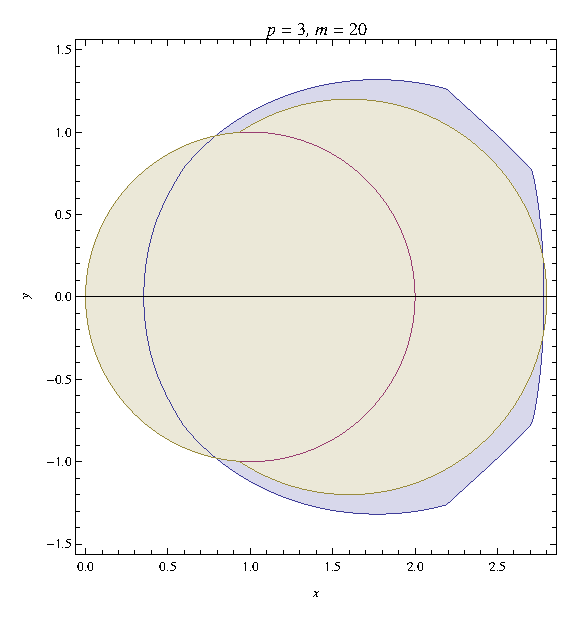
\includegraphics[width=0.3\textwidth]{fig_NM_PraConvReg_p3m20.eps}}
\subfigure[]{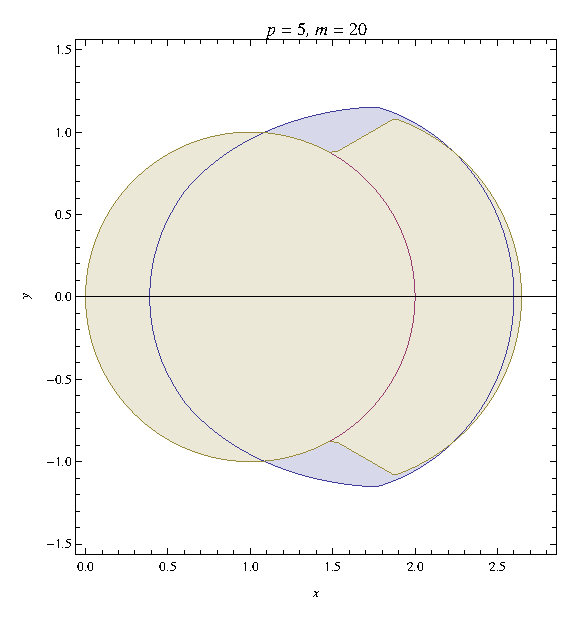
\includegraphics[width=0.3\textwidth]{fig_NM_PraConvReg_p5m20.eps}}
\subfigure[]{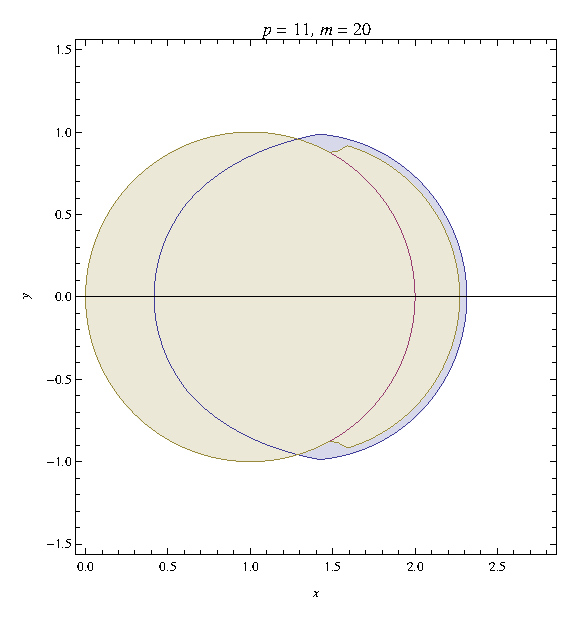
\includegraphics[width=0.3\textwidth]{fig_NM_PraConvReg_p11m20.eps}}\\
\subfigure[]{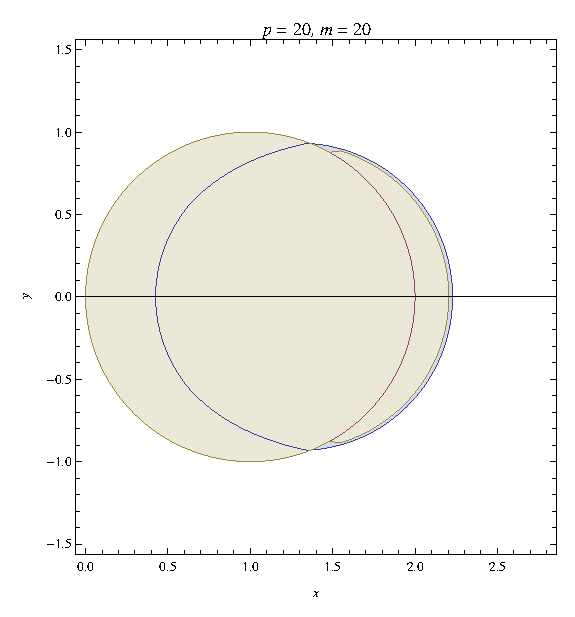
\includegraphics[width=0.3\textwidth]{fig_NM_PraConvReg_p20m20.eps}}
\subfigure[]{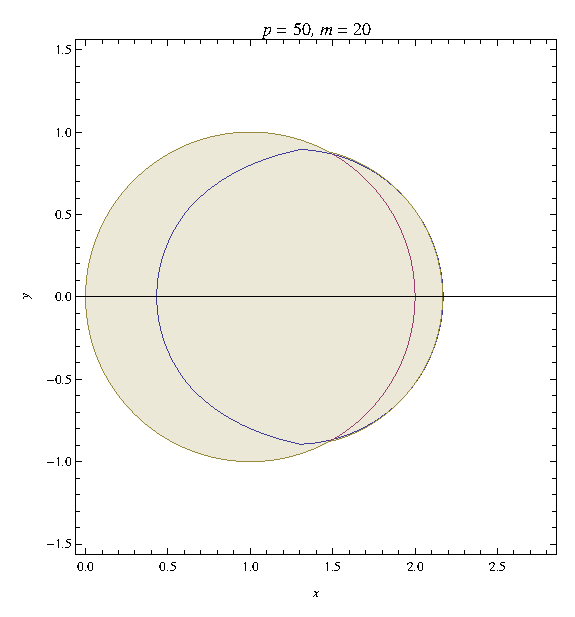
\includegraphics[width=0.3\textwidth]{fig_NM_PraConvReg_p50m20.eps}}
\subfigure[]{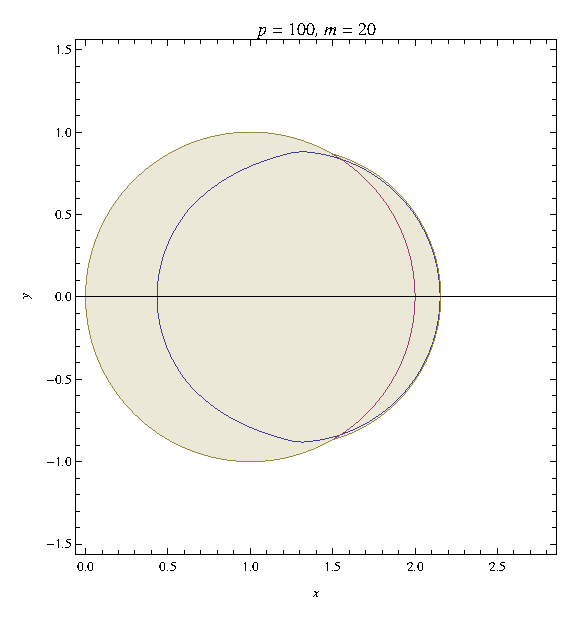
\includegraphics[width=0.3\textwidth]{fig_NM_PraConvReg_p100m20.eps}}\\
\caption{For fixed $m=20$ and $p=2,5,11,20,50,100$, the actual
convergence regions $\MCR_1$ defined in (\ref{set:R_NM}) (the union
of the red and blue parts) and the approximate convergence regions
$\MCR_1^{\text{N}}$ defined in (\ref{set:R_N_pra}) (the yellow
parts).}\label{fig:NM_PraConvReg}
\end{figure}








Next, we give some numerical examples to illustrate that the
convergence results obtained in Theorems \ref{th:MatrixNMCon} and
\ref{th:MatrixHMCon} are better than the existing ones. For
simplicity, in the following tests, we denote

\begin{enumerate}
\item
SN: Schur-Newton algorithm by choosing $\MCR_1^{\text{N}}$ defined
in (\ref{set:R_N_pra}) as the region $\MCR$ in step 2 and the
coupled Newton iteration (\ref{it:CoupledNM}) as the iterative
method in step 4;
\item
SN-old: Schur-Newton algorithm by choosing $\MCD_3$ defined in
(\ref{set:D3}) as the region $\MCR$ in step 2 and the coupled Newton
iteration (\ref{it:CoupledNM}) as the iterative method in step 4;
\item
SH: Schur-Halley algorithm by choosing $\MCR_2^{\text{H}}$ defined
in (\ref{set:R_H_pra}) as the region $\MCR$ in step 2 and the
coupled Halley iteration (\ref{it:CoupledHM}) as the iterative
method in step 4;
\item
SH-old: Schur-Halley algorithm by choosing the disk $\{z\in\CS:
|8/5-z|\leq1\}$ as the region $\MCR$ in step 2 and the coupled
Halley iteration (\ref{it:CoupledHM}) as the iterative method in
step 4.
\end{enumerate}
Recall that the convergence regions of SN-old and SH-old are
presented by Guo in \cite{Guo2010} and Iannazzo in
\cite{Iannazzo2008}, respectively. The iterations in the above four
algorithms are stopped when $\|N_k - \I\| < \sqrt{n}u/2$, where $n$
is the size of $A$ and $u = 2^{-52} \approx2.2204\me-16$.


Our numerical experiments were carried out in MATLAB 7.0 running on
a PC Intel Pentium P6200 of 2.13 GHz CPU. To measure of the quality
of a computed solution $X$, we use the relative residual $\rho_A(X)$
and relative error $\textup{err}(X)$ as follows:
\begin{equation}
\label{eq:RelResErr} \rho_A(X) = \frac{\|A - X^p\|}{\|X\| \|\sum_{j
= 0}^{p - 1} \tran{(X^{p - 1 - j})}\otimes X^j\|}, \ \ \
\textup{err}(X) = \frac{\|A - X^p\|}{\|A\|},
\end{equation}
where $\otimes$ denotes the Kronecker product and $\|\cdot\|$
denotes the Frobenius norm. Note that the relative residual
$\rho_A(X)$ (given in \cite{GuoHigham2006}) is more practically
useful definition of relative residual (e.g., for testing purposes)
than relative error and that the averaged CPU time computed by the
standard MATLAB function \textsf{cputime}. The averaged time was
computed by repeating 100 times for each test matrix. Moreover, we
use `iter' to stand for the number of the iterations.
